% !TeX root = ../main.tex

%%% Tables %%%

\begin{table}[ht]
\centering
\caption{Accuracies and run times for all models. All reported values are averages, and $\pm$ refers to the standard deviation. The run times heavily depend upon the optimization method.}
\scalebox{0.8}{
\begin{tabular}{ccccccc}
Model                       & \multicolumn{1}{c}{Train Time (m)} & \multicolumn{1}{c}{Dive Type} & \multicolumn{1}{c}{Subdive Type} & \multicolumn{1}{c}{Dive Accuracy} & \multicolumn{1}{c}{Subdive Accuracy}  \\ \hline
\multirow{5}{*}{CarHMM-DFT} & \multirow{5}{*}{$62 \pm 10$}   & Both                          & Both                             & -------------                     & $1.00 \pm 0.00$                       \\
                            &                                    & 1                             & 1                                & \multirow{2}{*}{-------------}    & $1.00 \pm 0.00$                       \\ 
                            &                                    & 1                             & 2                                &                                   & $1.00 \pm 0.00$                       \\ 
                            &                                    & 2                             & 1                                & \multirow{2}{*}{-------------}    & $1.00 \pm 0.00$                       \\ 
                            &                                    & 2                             & 2                                &                                   & $1.00 \pm 0.00$                       \\ \hline 
\multirow{5}{*}{HHMM-DFT}   & \multirow{5}{*}{$140 \pm 29$}   & Both                          & Both                             & $0.94 \pm 0.03$                   & $1.00 \pm 0.00$                       \\
                            &                                    & 1                             & 1                                & \multirow{2}{*}{$0.93\pm0.04$}    & $1.00 \pm 0.00$                       \\ 
                            &                                    & 1                             & 2                                &                                   & $1.00 \pm 0.00$                       \\ 
                            &                                    & 2                             & 1                                & \multirow{2}{*}{$0.94\pm0.03$}    & $1.00 \pm 0.00$                       \\ 
                            &                                    & 2                             & 2                                &                                   & $1.00 \pm 0.00$                       \\ \hline
\multirow{5}{*}{CarHHMM}    & \multirow{5}{*}{$258 \pm 82$}   & Both                          & Both                             & $0.87 \pm 0.11$                   & $0.89 \pm 0.01$                       \\
                            &                                    & 1                             & 1                                & \multirow{2}{*}{$0.79\pm0.23$}    & $0.43 \pm 0.08$                       \\ 
                            &                                    & 1                             & 2                                &                                   & $1.00 \pm 0.00$                       \\ 
                            &                                    & 2                             & 1                                & \multirow{2}{*}{$0.96\pm0.03$}    & $0.82 \pm 0.01$                       \\ 
                            &                                    & 2                             & 2                                &                                   & $1.00 \pm 0.00$                       \\ \hline
\multirow{5}{*}{CarHHMM-DFT}& \multirow{5}{*}{$150 \pm 37$}   & Both                          & Both                             & $0.94 \pm 0.03$                   & $1.00 \pm 0.00$                       \\
                            &                                    & 1                             & 1                                & \multirow{2}{*}{$0.93\pm0.04$}    & $1.00 \pm 0.00$                       \\ 
                            &                                    & 1                             & 2                                &                                   & $1.00 \pm 0.00$                       \\ 
                            &                                    & 2                             & 1                                & \multirow{2}{*}{$0.94\pm0.03$}    & $1.00 \pm 0.00$                       \\ 
                            &                                    & 2                             & 2                                &                                   & $1.00 \pm 0.00$                       \\ \hline
\end{tabular}
}
\label{table:accuracy}
\end{table}

\begin{table}[ht]
    \centering
    \caption{Estimates and standard errors of emission parameters for killer whale data under the CarHHMM-DFT.}
    \scalebox{0.75}{
\begin{tabular}{ccccc}
    \multirow{2}{*}{Feature}                                                       & \multirow{2}{*}{Dive / Subdive Type} & \multicolumn{3}{c}{Parameter Estimate}              \\
                                                                                   &                                      & $\hat \mu$      & $\hat \sigma$   & $\hat \phi$     \\ \hline
    \multirow{2}{*}{Dive Duration $(s)$ - $Y$}                                     & 1                                    & $25.687 \pm 0.602$ & $9.573 \pm 0.514$ & ---             \\
                                                                                   & 2                                    & $104.601 \pm 9.395$ & $64.678 \pm 7.468$ & ---             \\ \hline
    \multirow{3}{*}{x-acceleration $(m/s^2)$ - $\left(\mathbf{Z}^{*(1)}\right)_x$} & 1                                    & $0.020 \pm 0.042$ & $0.034 \pm 0.001$ & $0.976 \pm 0.007$ \\
                                                                                   & 2                                    & $0.244 \pm 0.013$ & $0.079 \pm 0.001$ & $0.886 \pm 0.005$ \\
                                                                                   & 3                                    & $0.218 \pm 0.028$ & $0.265 \pm 0.007$ & $0.626 \pm 0.029$ \\ \hline
    \multirow{3}{*}{y-acceleration $(m/s^2)$ - $\left(\mathbf{Z}^{*(1)}\right)_y$} & 1                                    & $0.469 \pm 0.052$ & $0.044 \pm 0.001$ & $0.976 \pm 0.009$ \\
                                                                                   & 2                                    & $0.436 \pm 0.014$ & $0.082 \pm 0.001$ & $0.886 \pm 0.012$ \\
                                                                                   & 3                                    & $0.384 \pm 0.033$ & $0.321 \pm 0.009$ & $0.626 \pm 0.034$ \\ \hline
    \multirow{3}{*}{z-acceleration $(m/s^2)$ - $\left(\mathbf{Z}^{*(1)}\right)_z$} & 1                                    & $-0.683 \pm 0.061$ & $0.052 \pm 0.001$ & $0.976 \pm 0.005$ \\
                                                                                   & 2                                    & $-0.593 \pm 0.016$ & $0.096 \pm 0.001$ & $0.886 \pm 0.009$ \\
                                                                                   & 3                                    & $-0.366 \pm 0.033$ & $0.317 \pm 0.009$ & $0.626 \pm 0.033$ \\ \hline
    \multirow{3}{*}{Fourier sum - $Z^{*(2)}$}                                      & 1                                    & $23.340 \pm 0.282$ & $12.948 \pm 0.269$ & ---             \\
                                                                                   & 2                                    & $301.189 \pm 3.244$ & $330.050 \pm 4.166$ & ---             \\
                                                                                   & 3                                    & $10204.010 \pm 211.242$ & $15299.066 \pm 352.674$ & ---             \\ \hline
    \end{tabular}
    }
    \label{table:emis_dists_CarHHMM-DFT}
\end{table}

%%% model definitions %%%

\begin{figure}[ht]
    \begin{subfigure}{\textwidth}
      \centering
      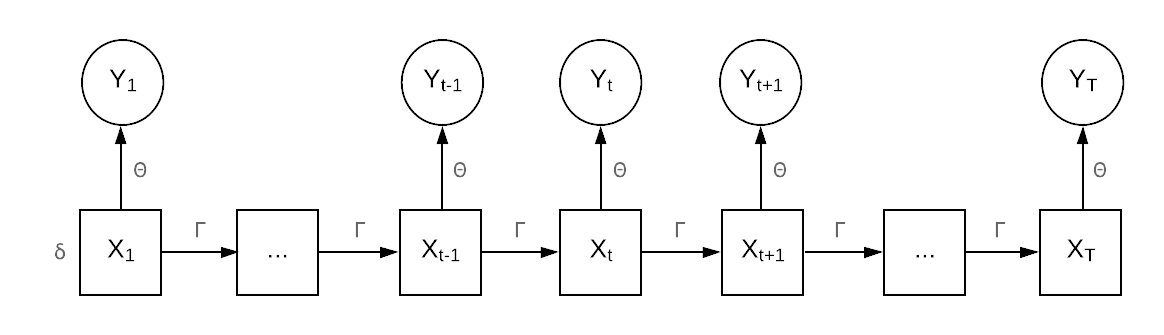
\includegraphics[width=4in]{../Plots/HMM.png}  
      \caption{Hidden Markov Model (\textbf{HMM})}
      \label{fig:HMM}
    \end{subfigure}
    %
    \newline
    %
    \begin{subfigure}{\textwidth}
      \centering
      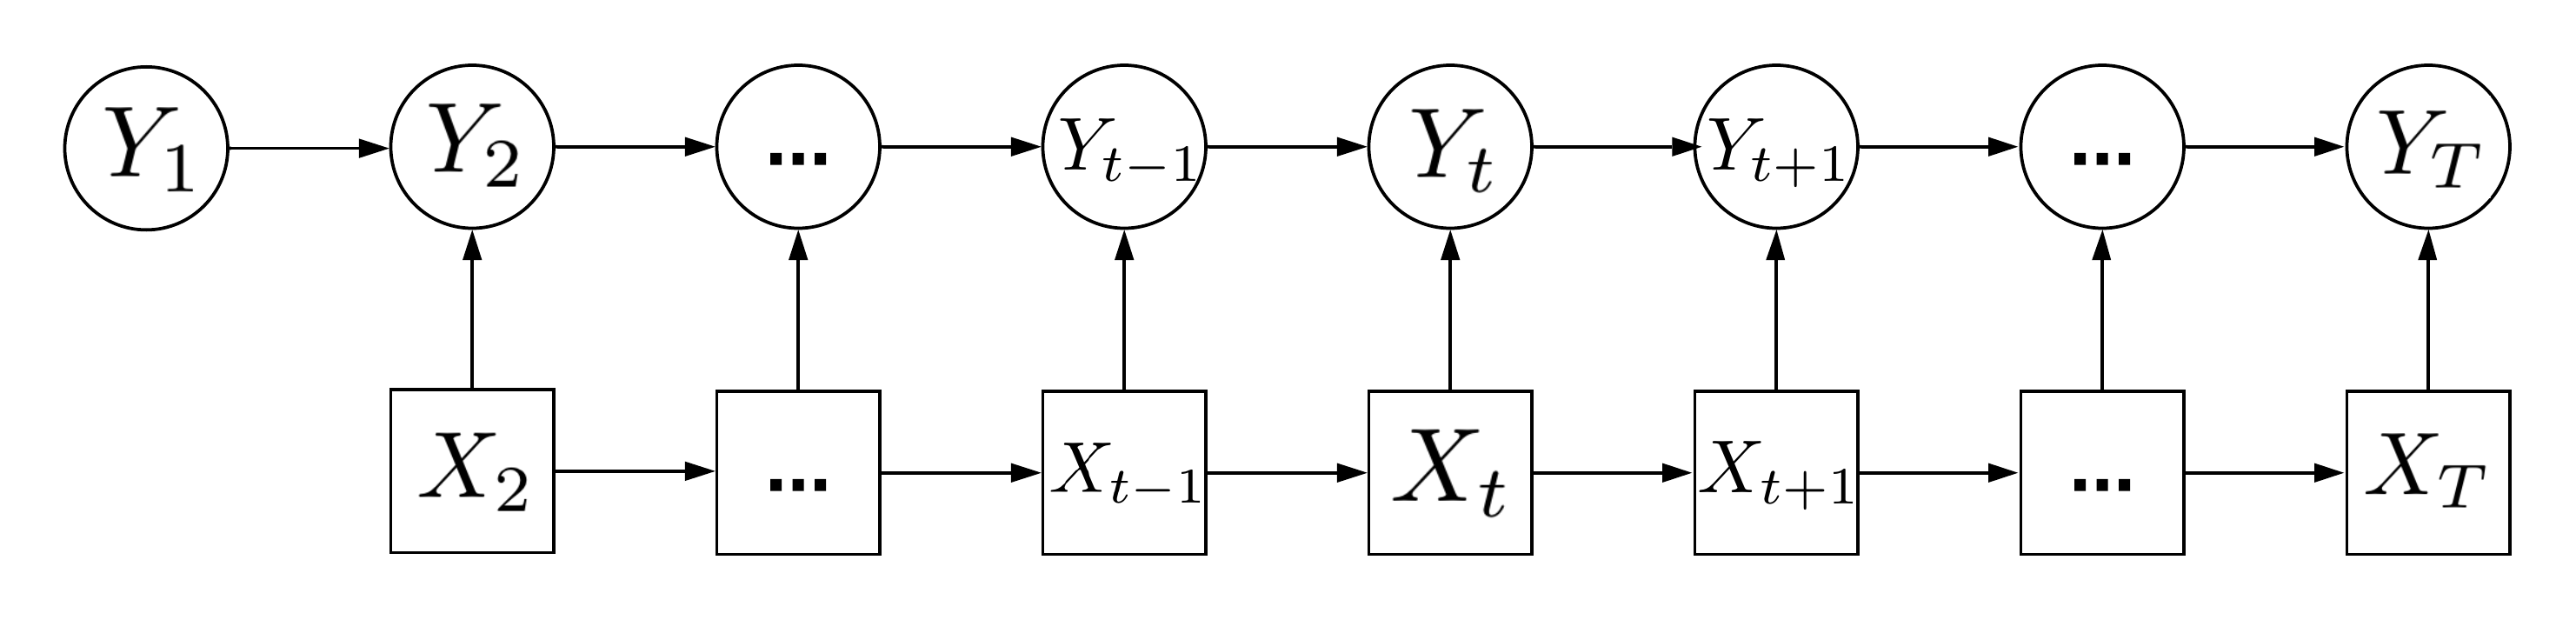
\includegraphics[width=4in]{../Plots/CarHMM.png}  
      \caption{Conditionally Auto-regressive HMM (\textbf{CarHMM})}
      \label{fig:CarHMM}
    \end{subfigure}
    %
    \newline
    %
    \begin{subfigure}{\textwidth}
      \centering
      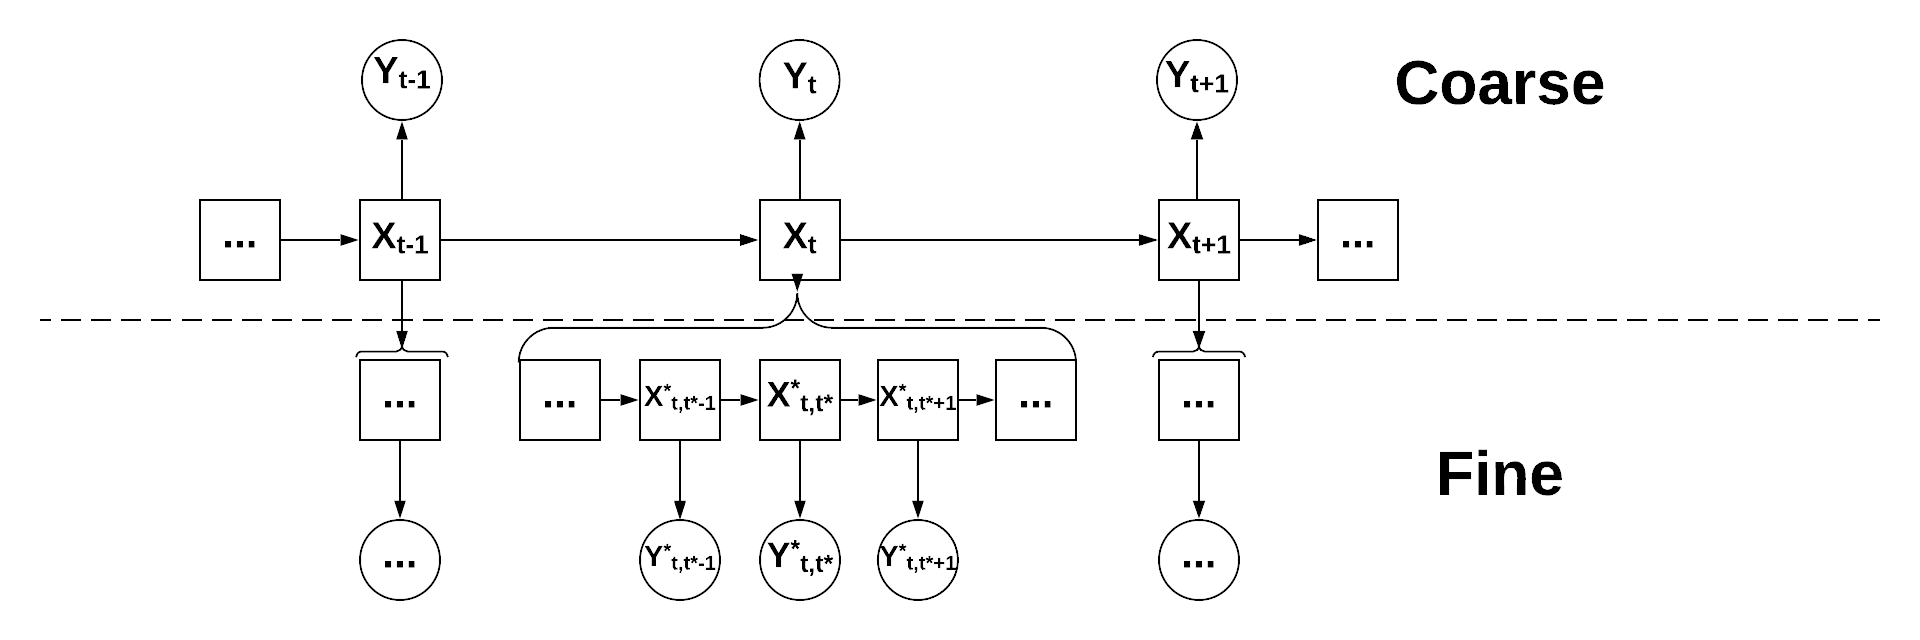
\includegraphics[width=4in]{../Plots/HHMM.png}  
      \caption{Hierarchical HMM (\textbf{HHMM})}
      \label{fig:HHMM}
    \end{subfigure}
    %
    \newline
    %
    \begin{subfigure}{\textwidth}
      \centering
      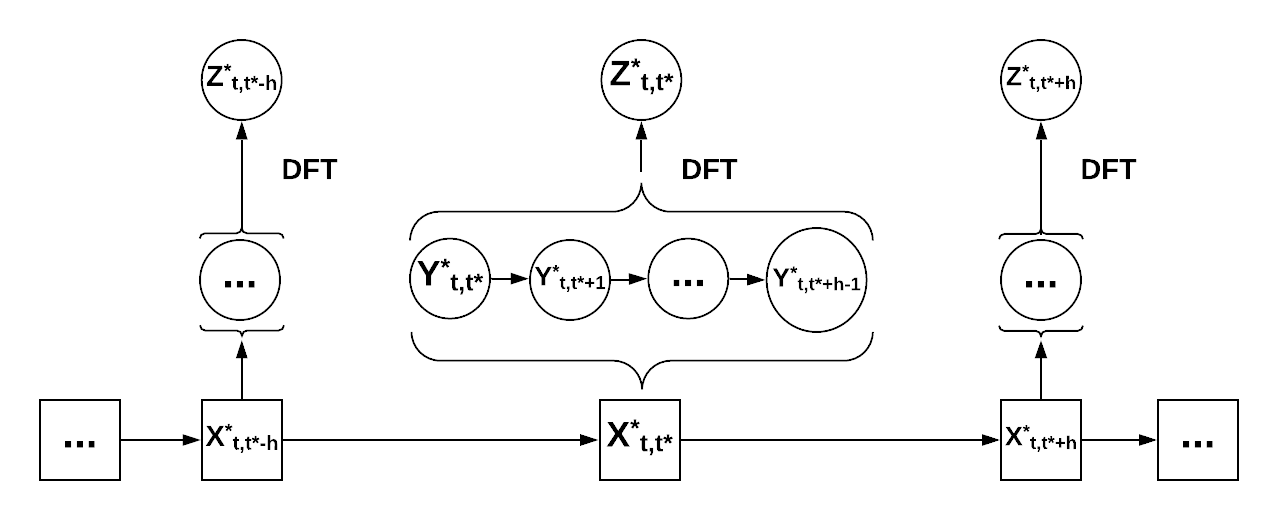
\includegraphics[width=4in]{../Plots/HMM-DFT.png}  
      \caption{HMM with Discrete Fourier Transform (\textbf{HMM-DFT})}
      \label{fig:HMM-DFT}
    \end{subfigure}
    \caption{Graphical representations of HMM models}
    \label{fig:models}
\end{figure}

%%% simulation study %%%

\begin{figure}[ht]
	\centering
	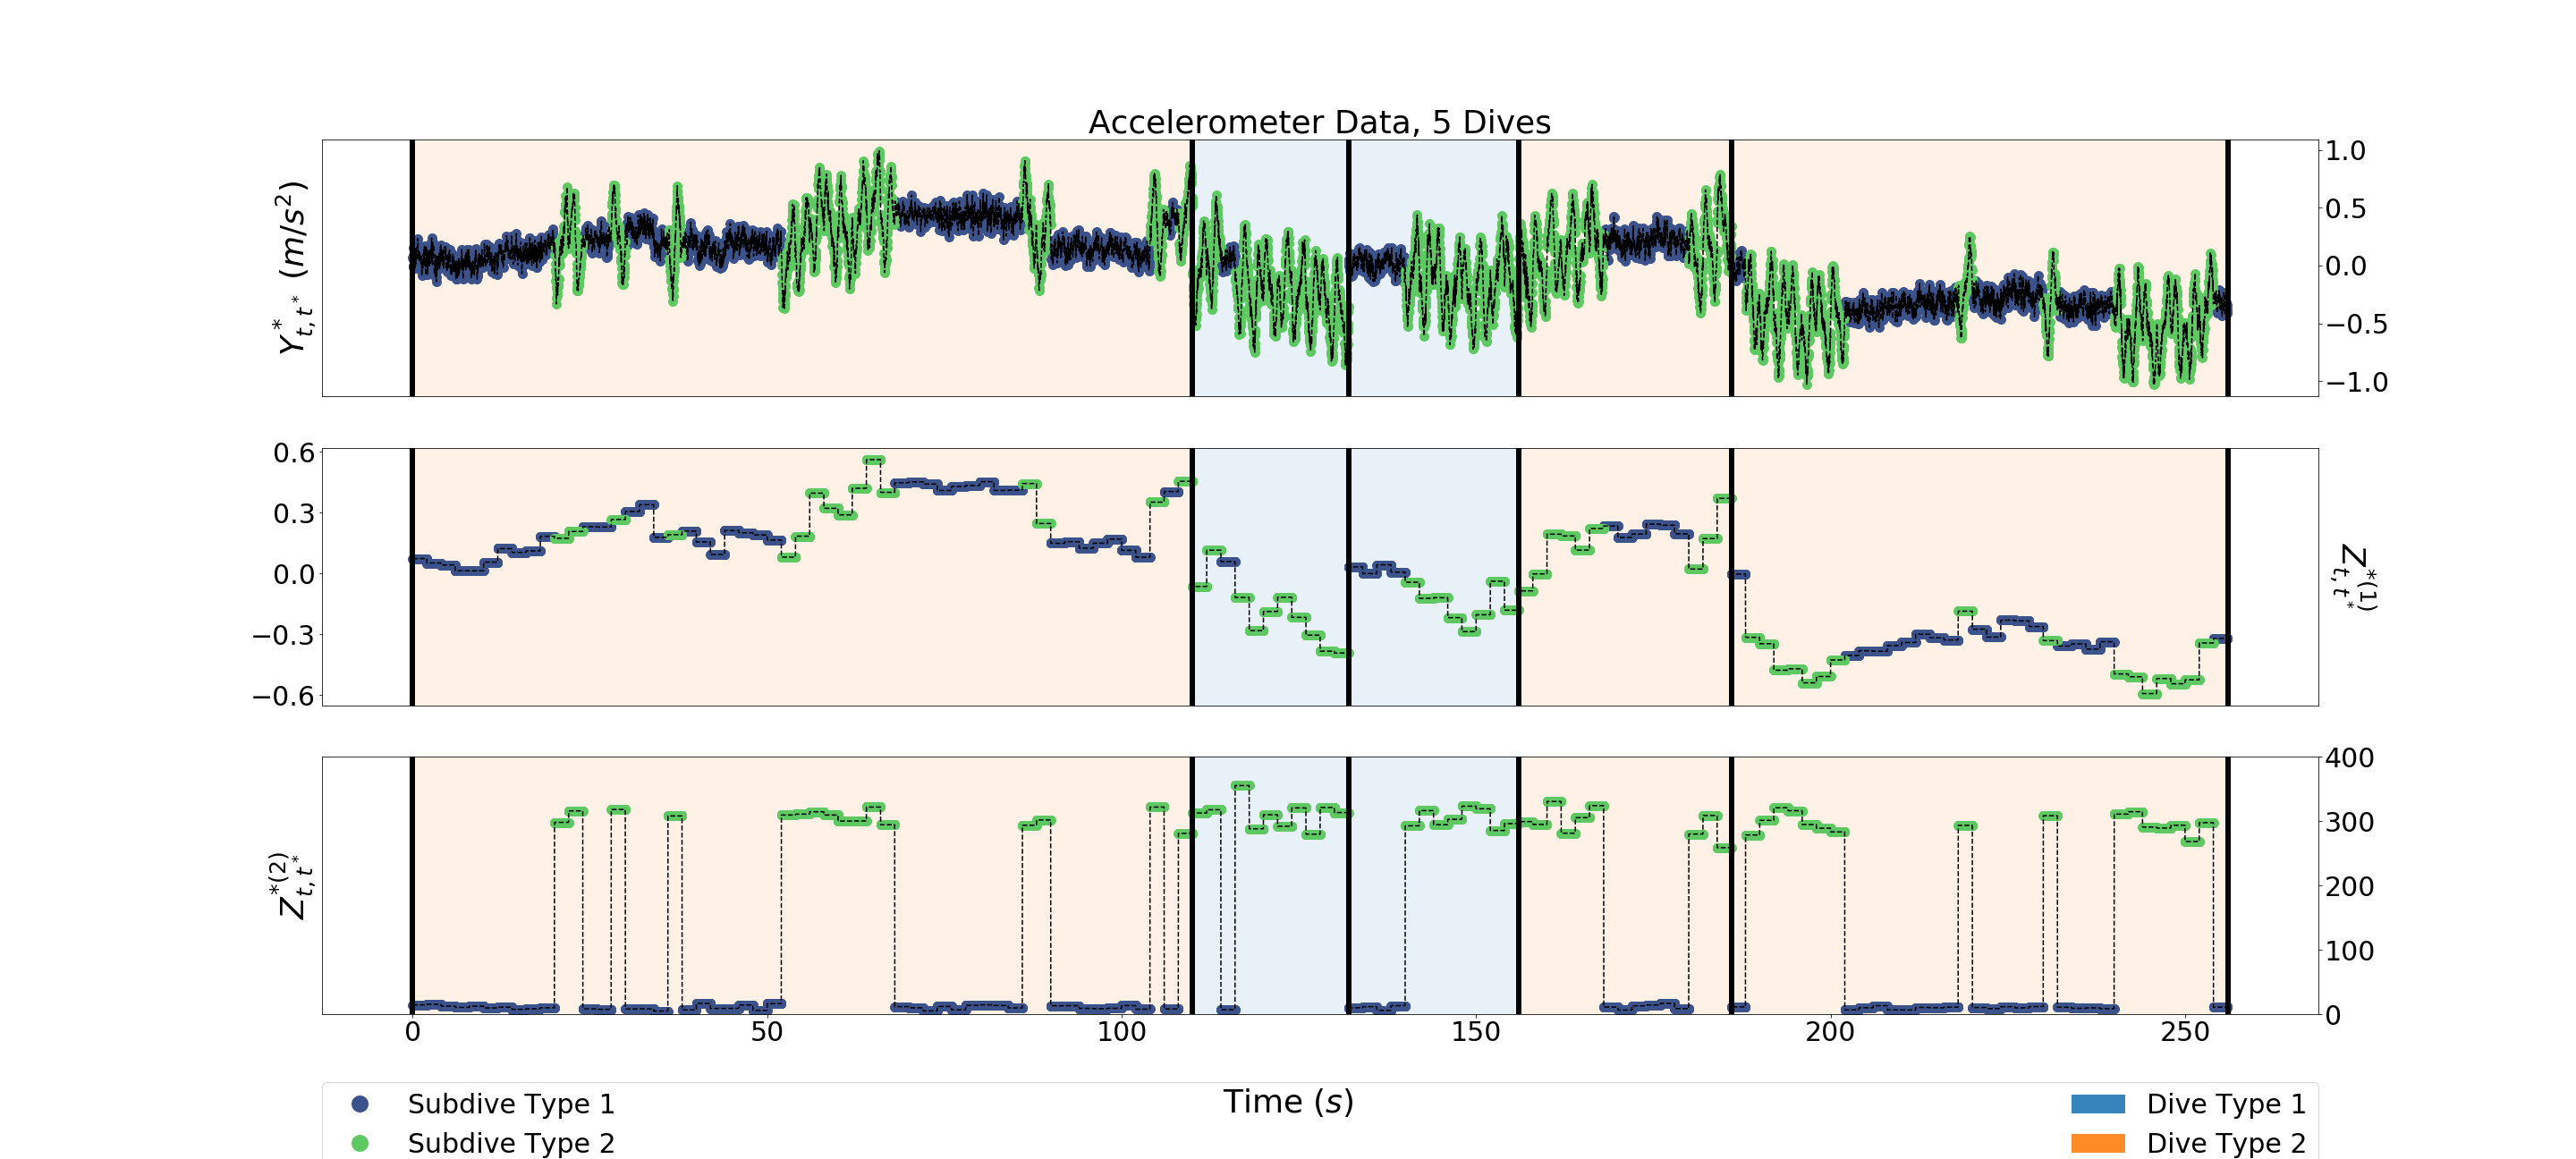
\includegraphics[width=5in]{../Plots/sim_data.png}
	\caption{Simulated acceleration data for one dive. The color of the line corresponds to the true fine-scale state of the subdive process, while the color of the background corresponds to the true dive type of the simulated whale.}
	\label{fig:sim_data}
\end{figure}

\begin{figure}[ht]
	\centering
	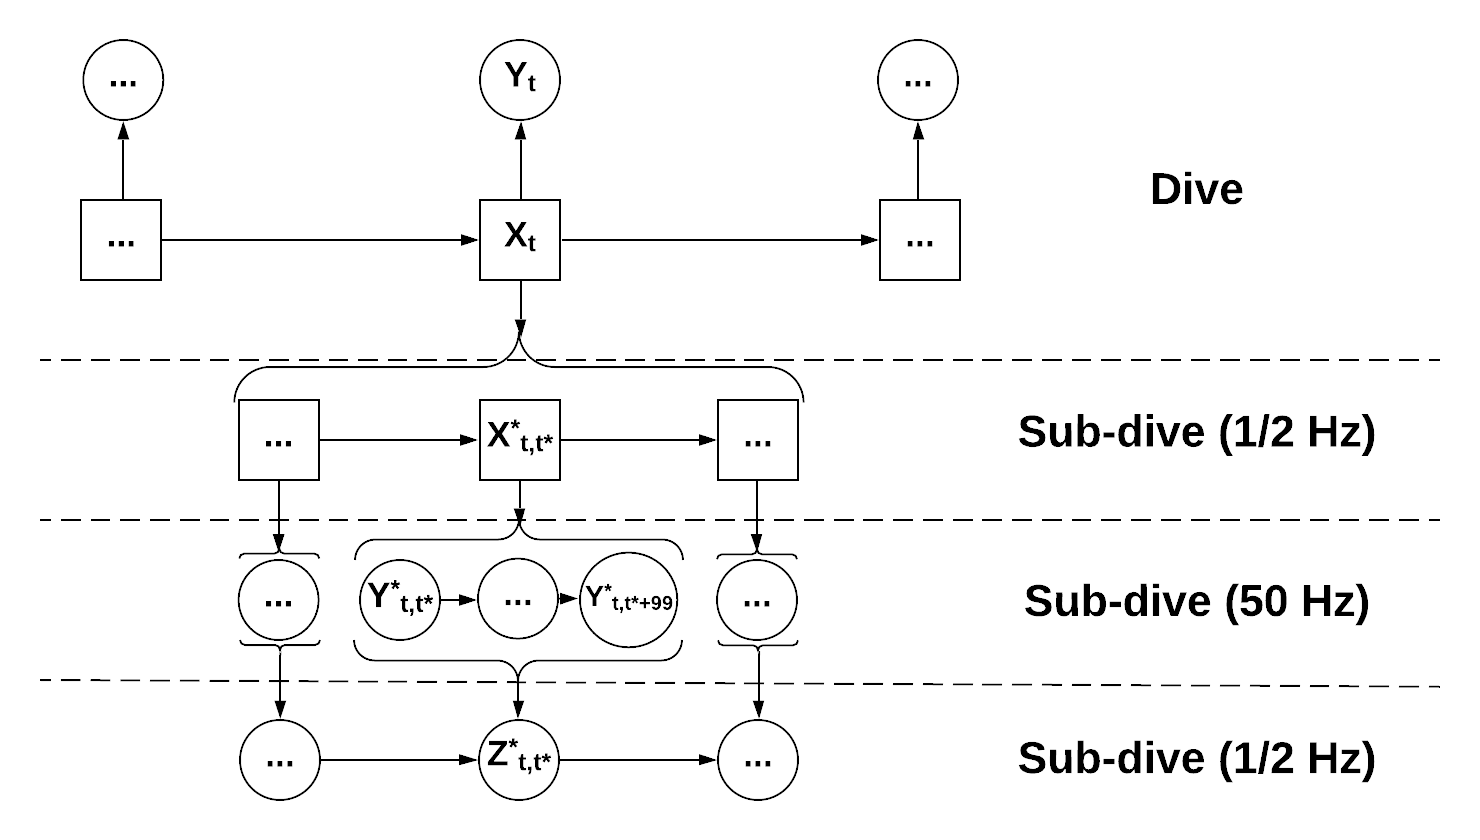
\includegraphics[width=5in]{../Plots/CarHHMM-DFT.png}
	\caption{Graphical representation the model used in the simulation and case study, the \textbf{CarHHMM-DFT}.}
	\label{fig:CarHHMM-DFT}
\end{figure}

\begin{figure}[ht]
    \centering
    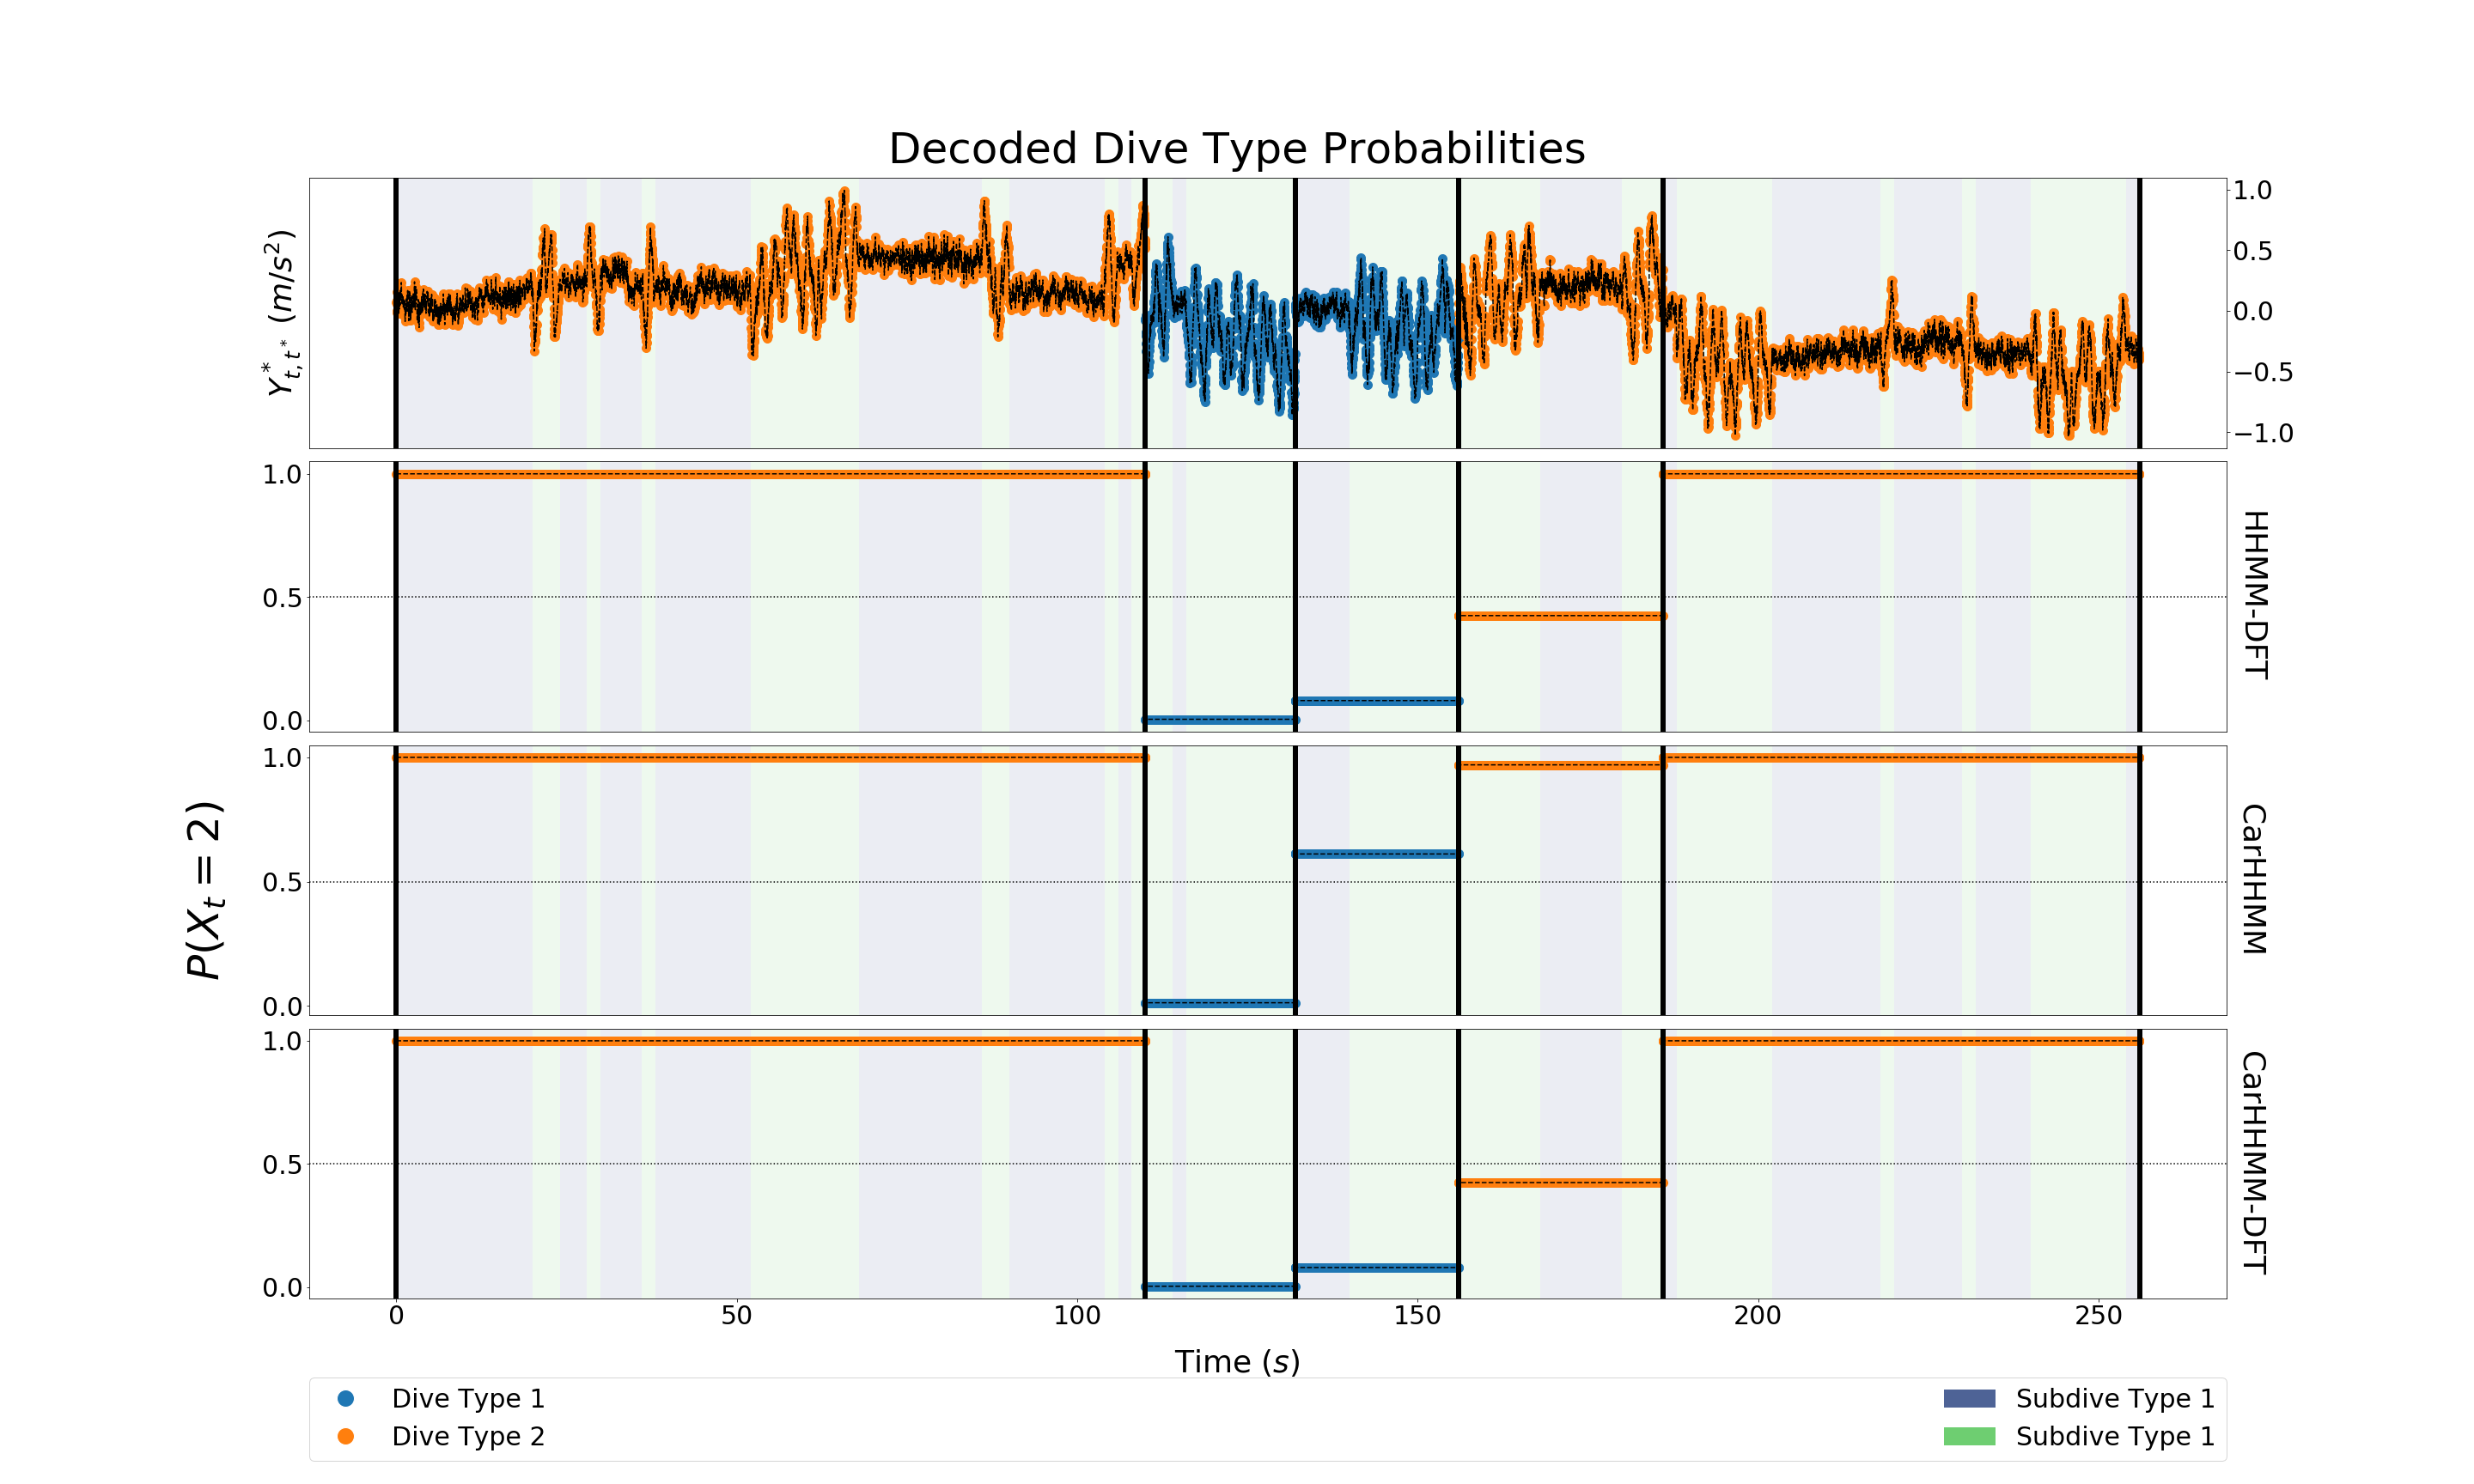
\includegraphics[width=5in]{../Plots/Posterior_Coarse_States.png}
    \caption{Decoded probabilities of each dive type for 5 dives of one simulated data set. The colors correspond to the true dive or subdive type}
    \label{fig:acc_coarse}
\end{figure}

\begin{figure}[ht]
    \centering
    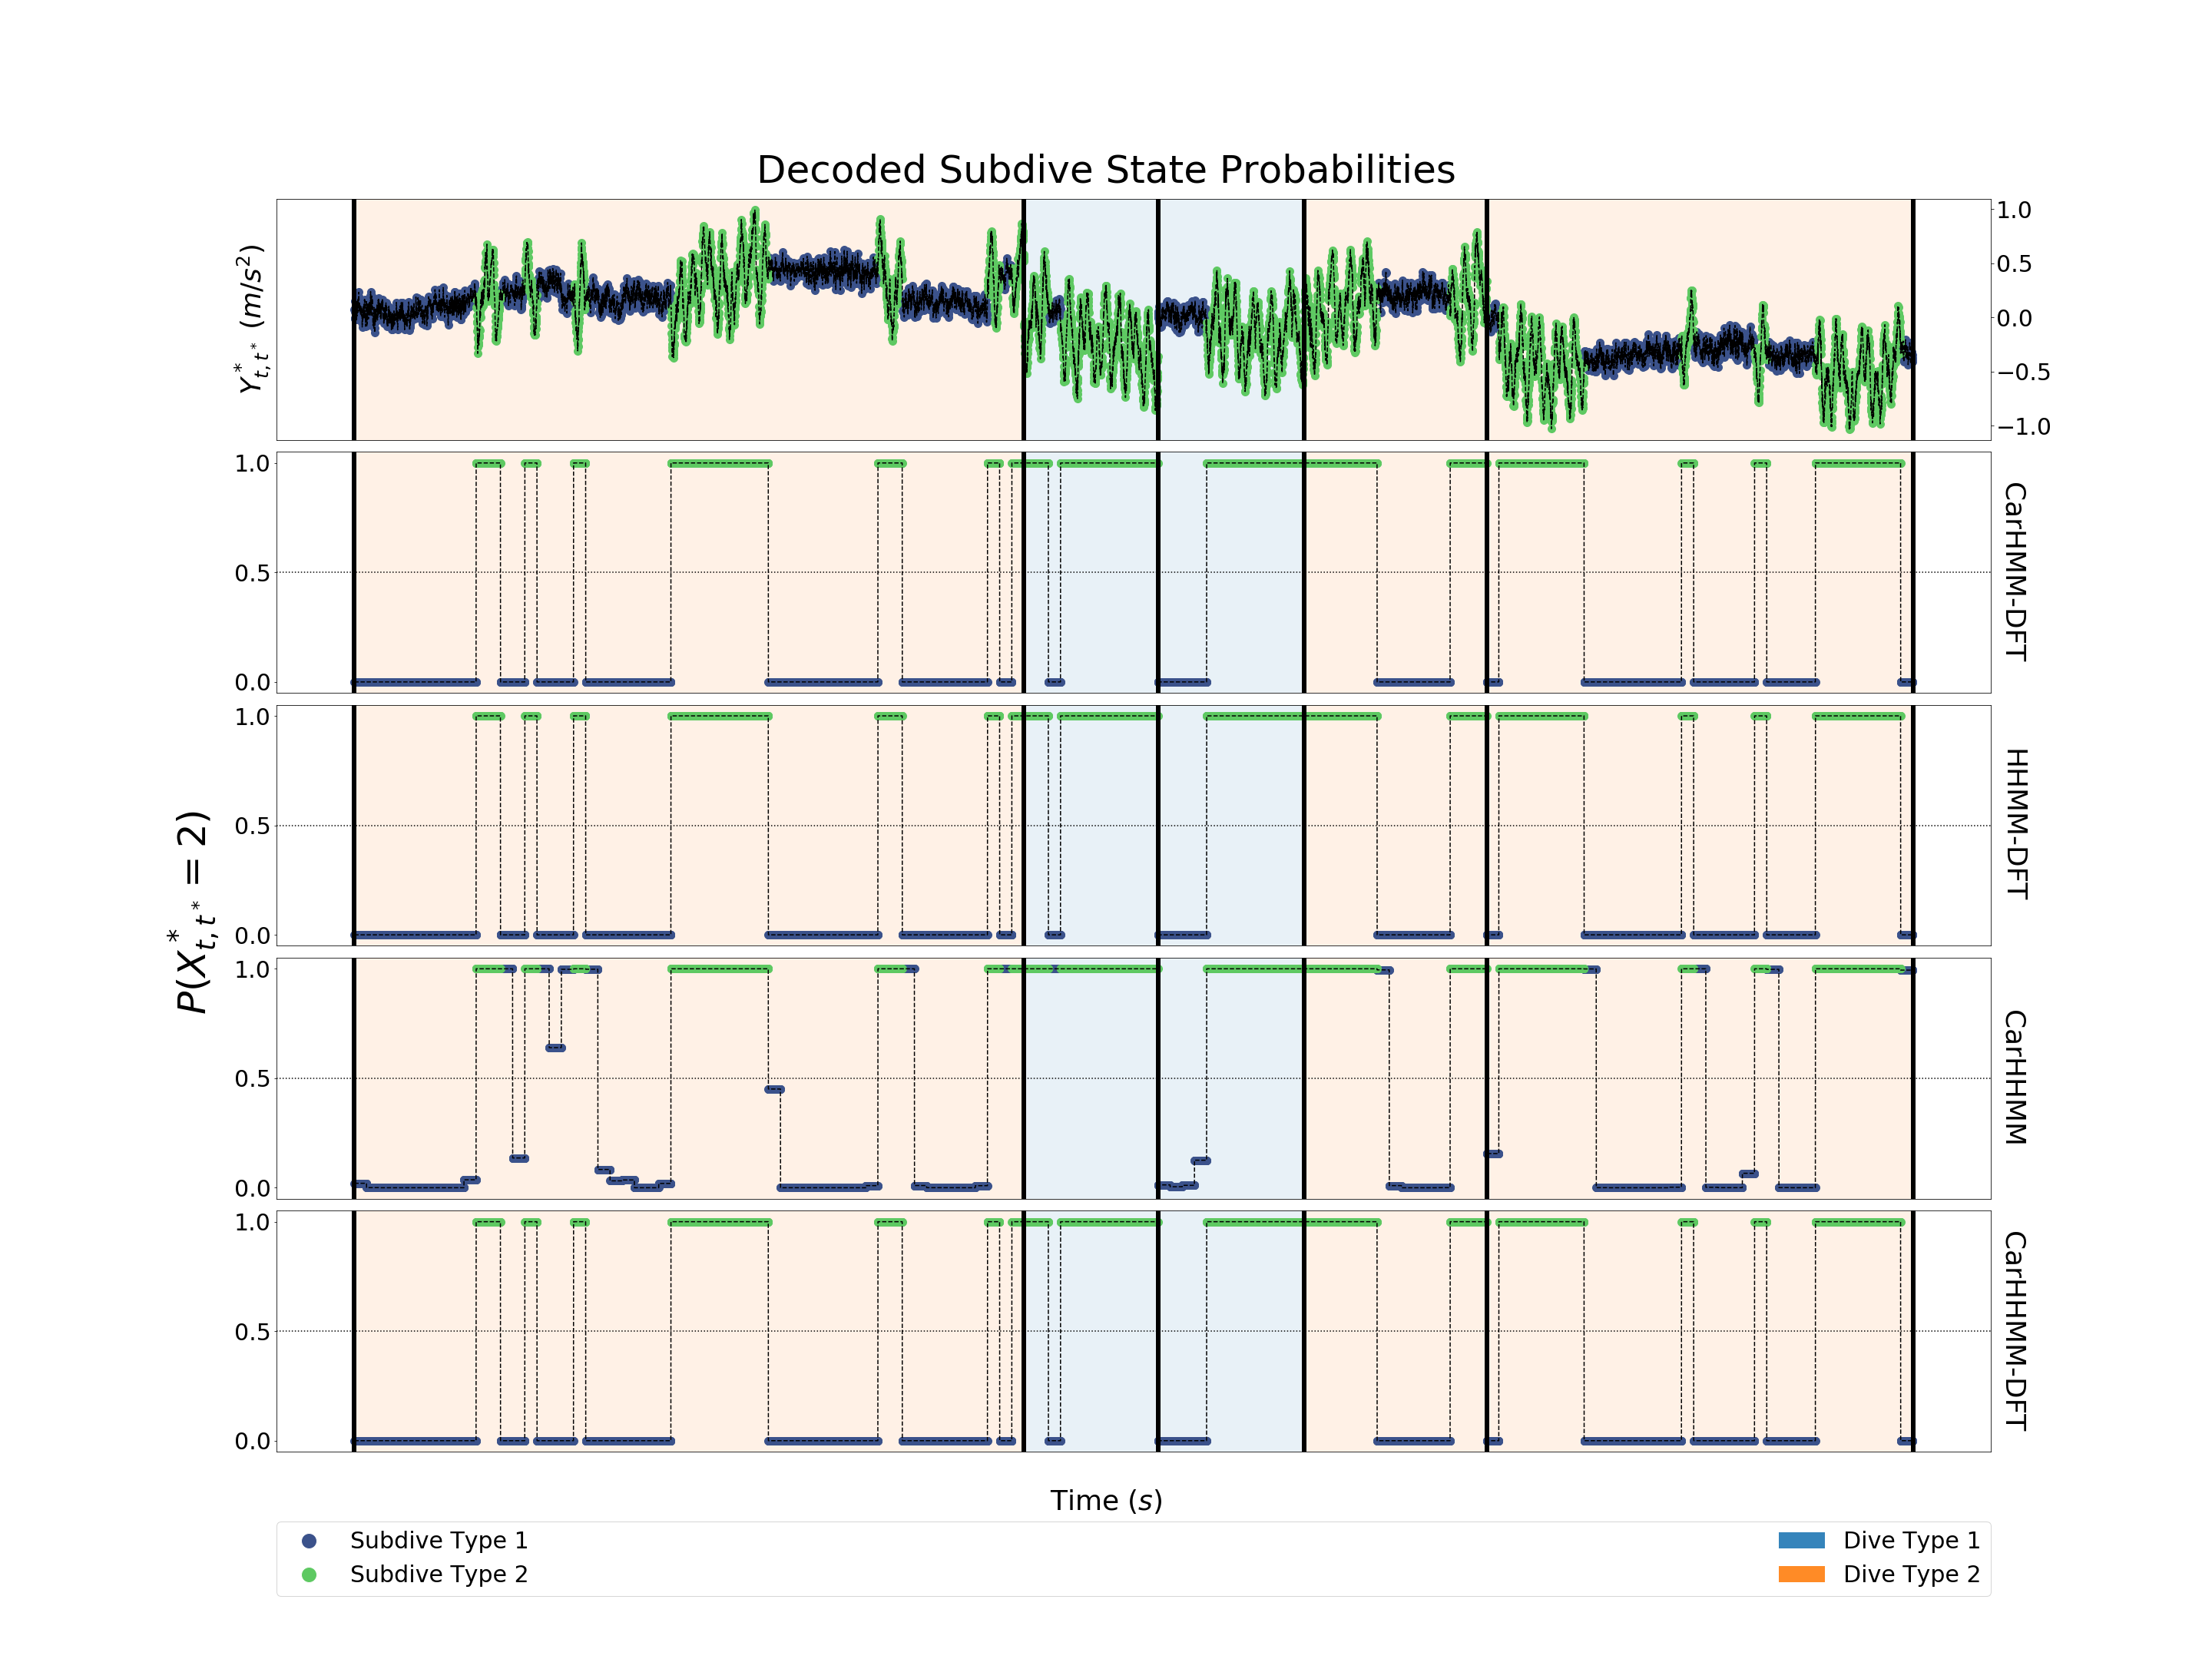
\includegraphics[width=5in]{../Plots/Posterior_Fine_States.png}
    \caption{Decoded probabilities of each subdive type for 5 dives of one simulated data set. The colors correspond to the true dive or subdive type}
    \label{fig:acc_fine}
\end{figure}

%%% Case Study %%%

\begin{figure}[ht]
	\centering
	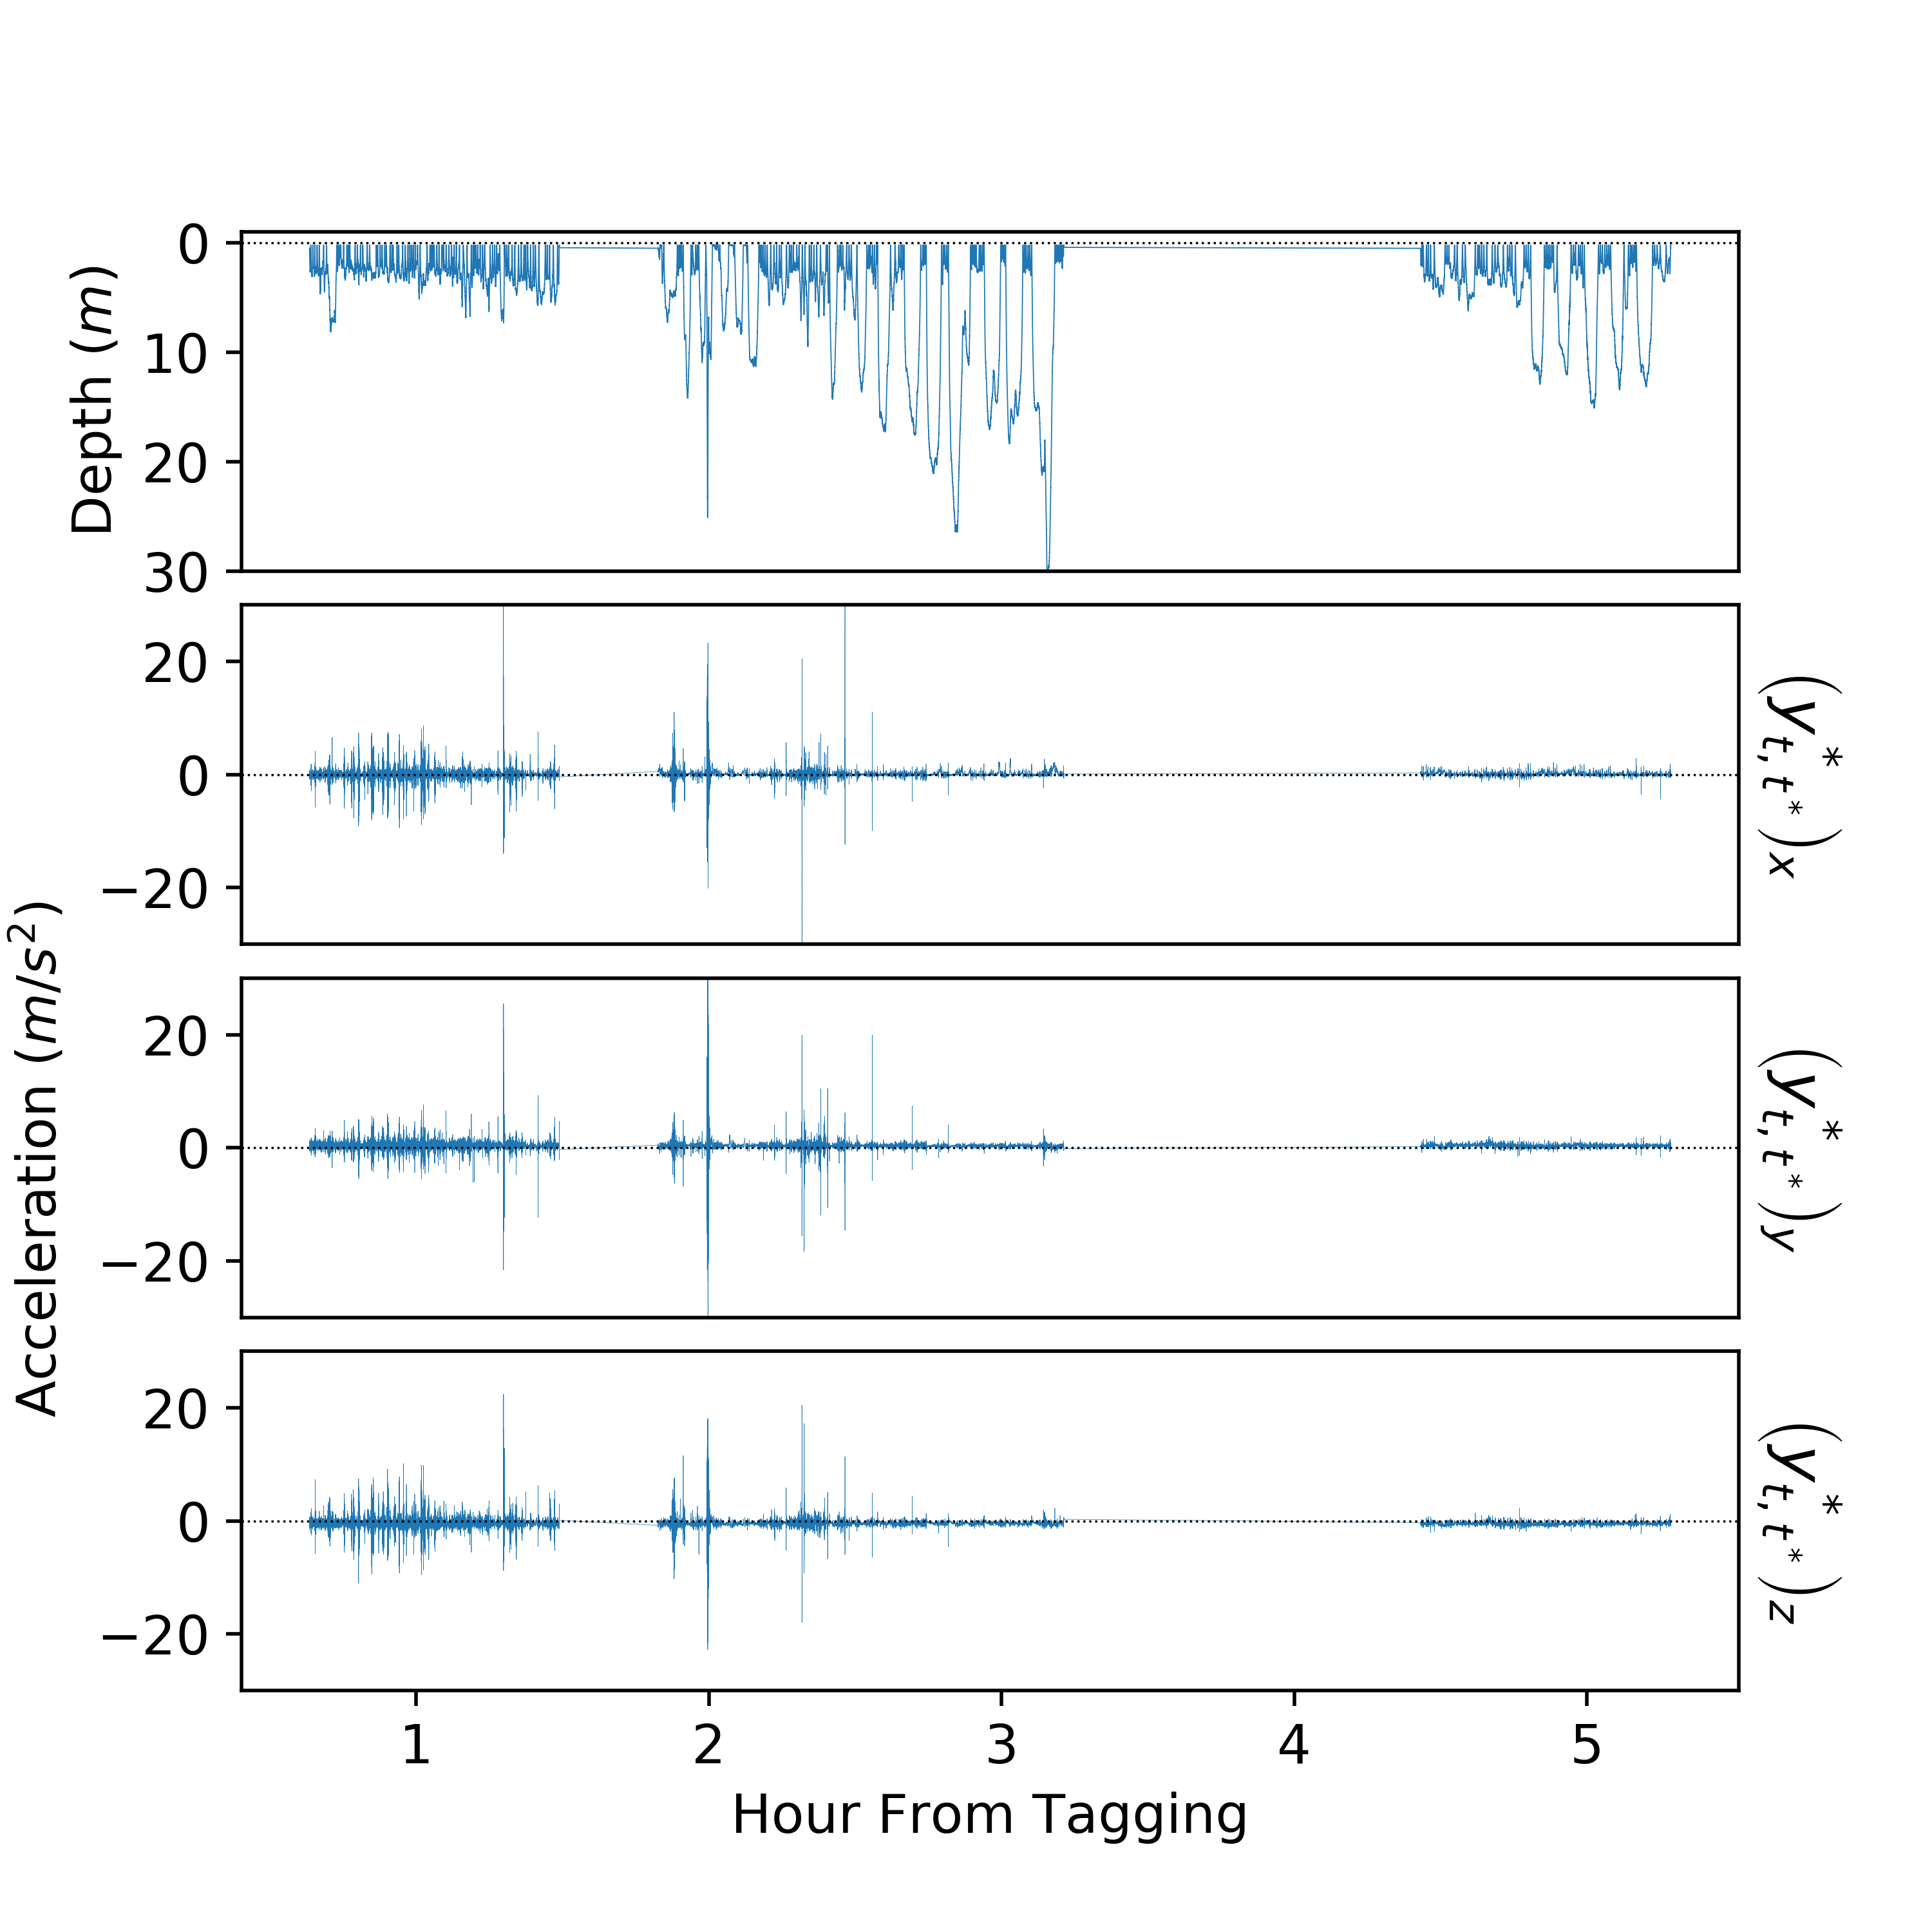
\includegraphics[width=5in]{../Plots/raw_data.png}
	\caption{Dive depth (top panel) and acceleration (bottom three panels) as functions of time, from the killer whale data set}
	\label{fig:data}
\end{figure}

\begin{figure}[ht]
	\centering
	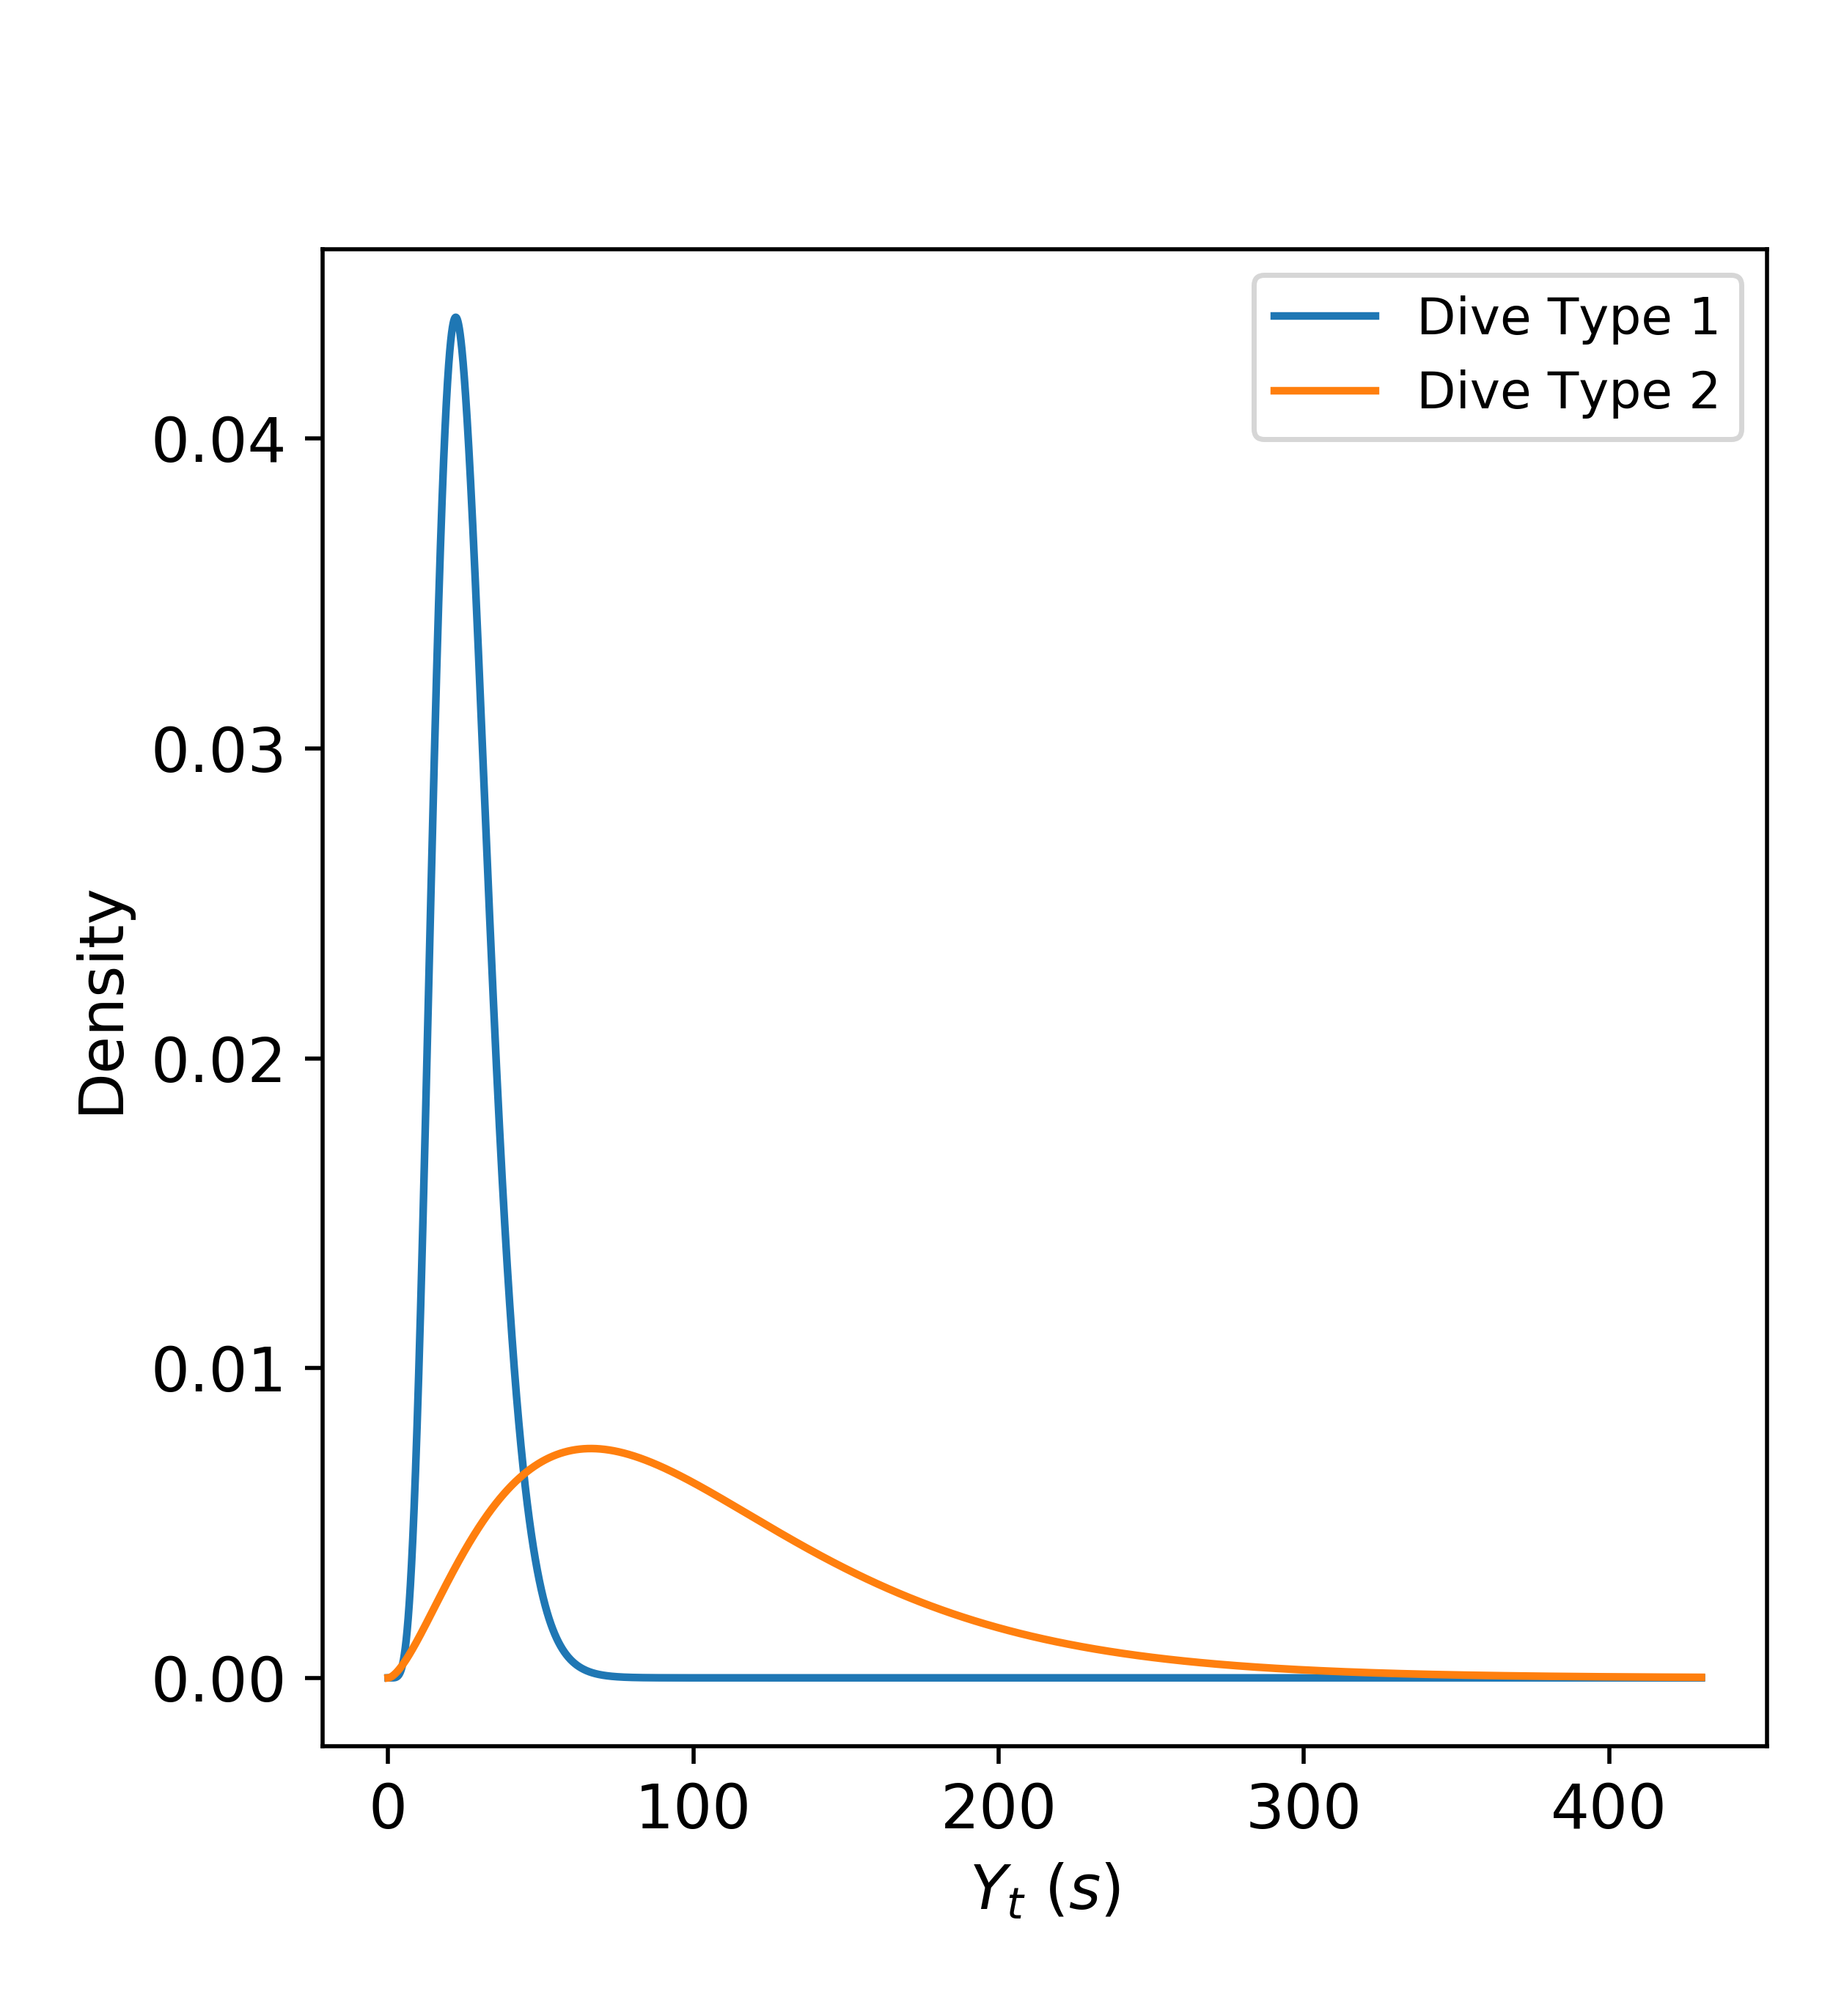
\includegraphics[width=5in]{../Plots/CarHHMM2-coarse-emissions.png}
	\caption{Estimated probability distributions for each coarse-scale observation in each dive type.}
	\label{fig:coarse_emis}
\end{figure}

\begin{figure}[ht]
	\centering
	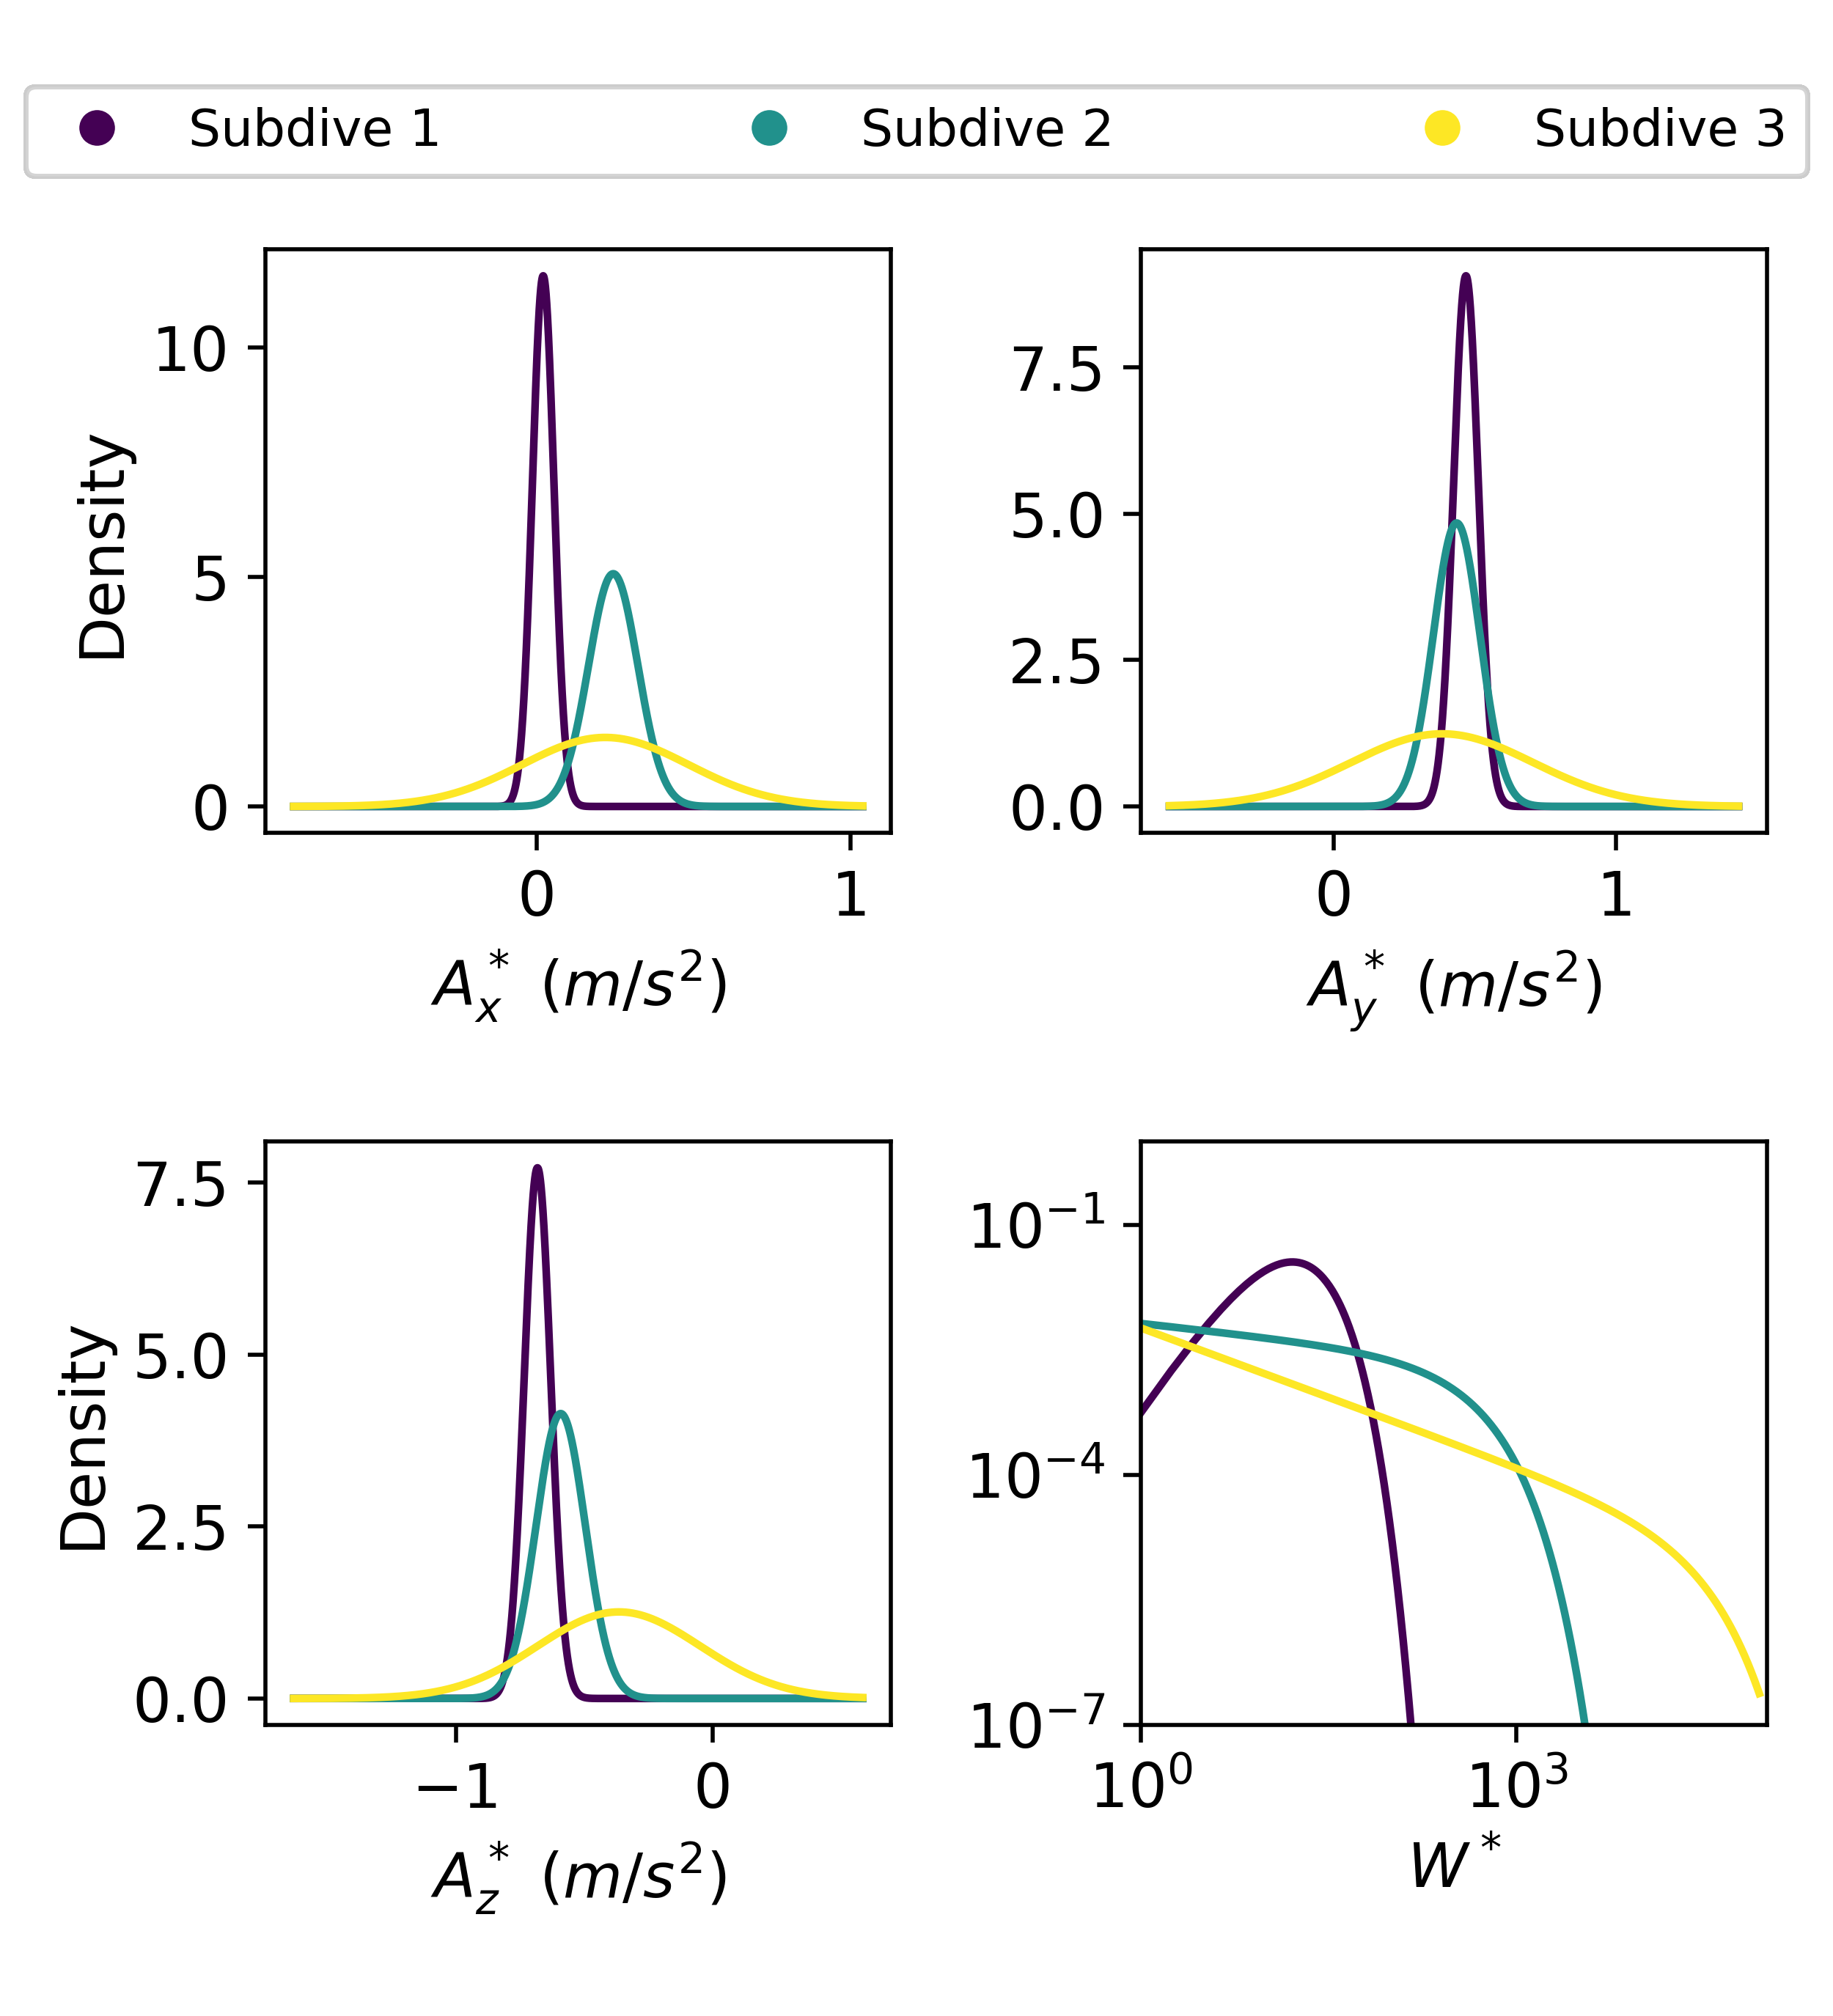
\includegraphics[width=5in]{../Plots/CarHHMM2-fine-emissions.png}
	\caption{Estimated probability distributions for each fine-scale observation in each behavioral state. Note that the distributions of acceleration do not take auto-correlation into account (see Table \ref{table:emis_dists_CarHHMM-DFT})}
	\label{fig:fine_emis}
\end{figure}

\begin{figure}[ht]
	\centering
	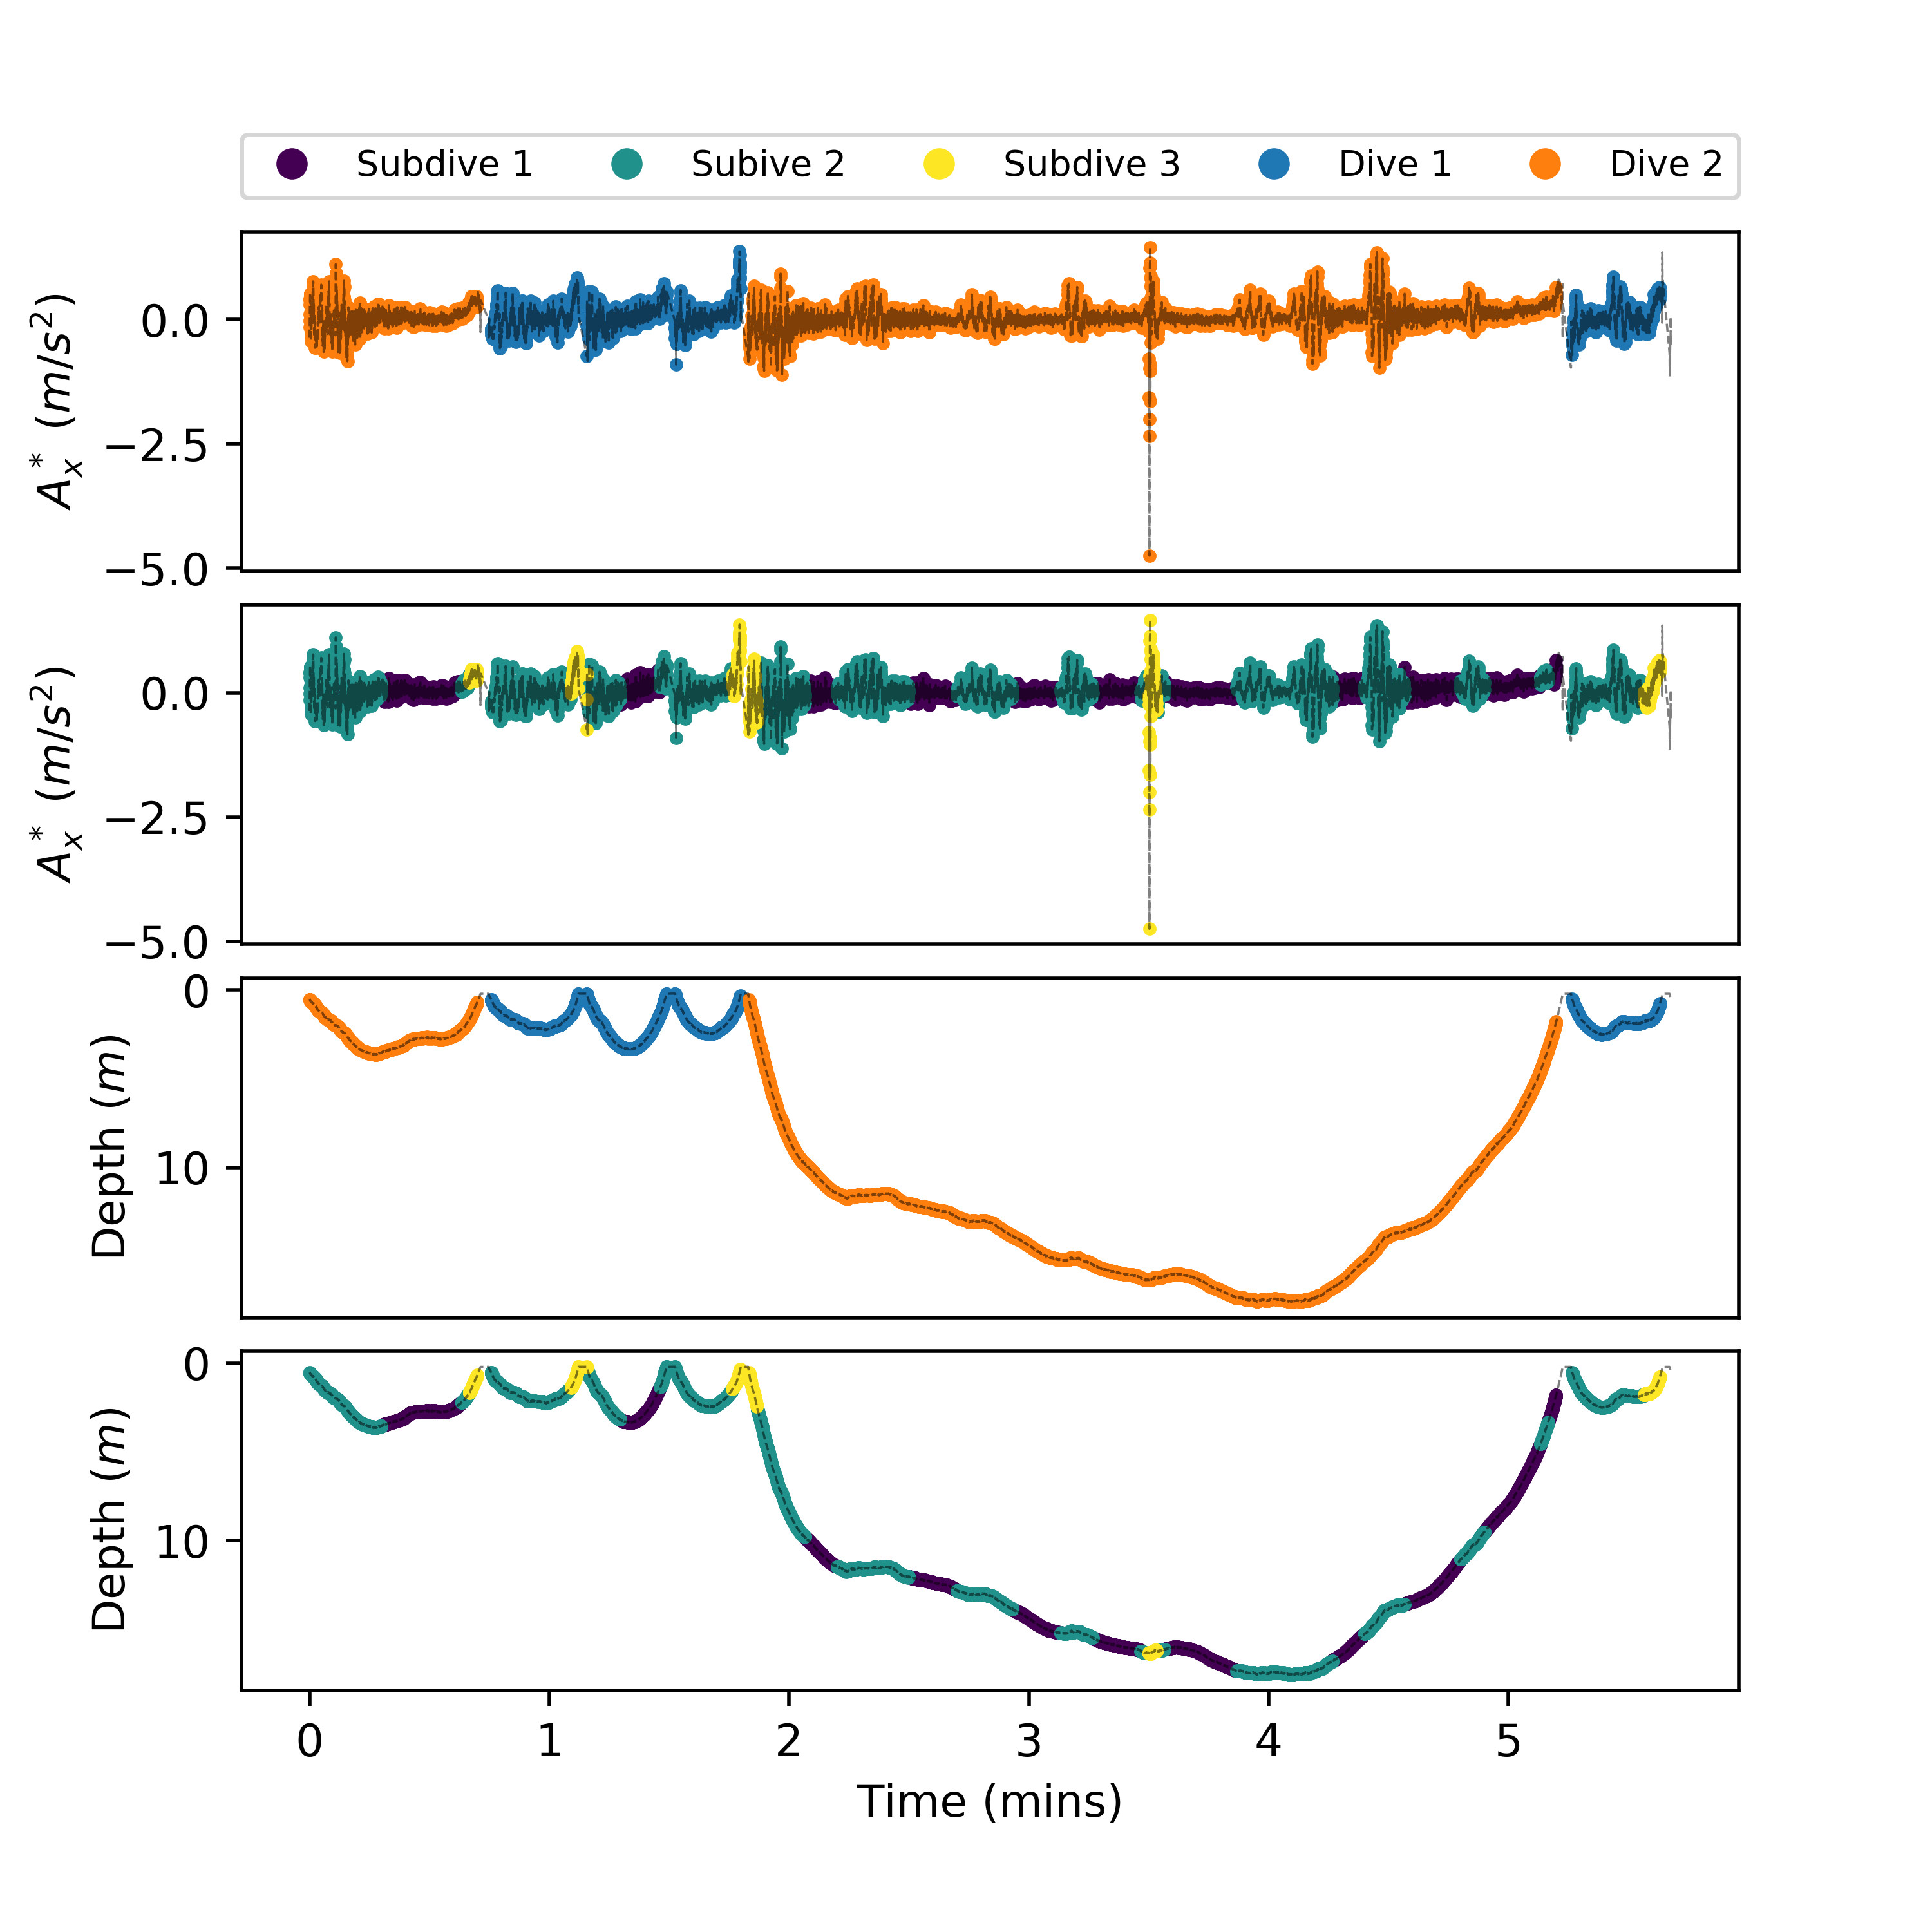
\includegraphics[width=5in]{../Plots/CarHHMM2_decoded_dives.png}
	\caption{Features of a particular set of killer whale dives and decoded estimates for the intra-dive behavioral states. The color of the plot corresponds to the behavioral or dive state with the highest probability.}
	\label{fig:labeled_dives}
\end{figure}

\begin{figure}[ht]
    \begin{subfigure}{0.45\textwidth}
    	\centering
    	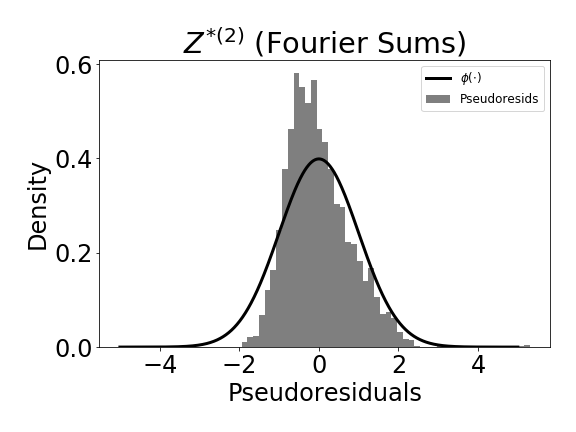
\includegraphics[width=2.25in]{../Plots/CarHHMM2_psedoresids_ahat.png}
    	\caption{Pseudoresiduals of $Z^{*(2)}$}
    	\label{fig:pseudoresids}
    \end{subfigure}
    \begin{subfigure}{0.45\textwidth}
    	\centering
    	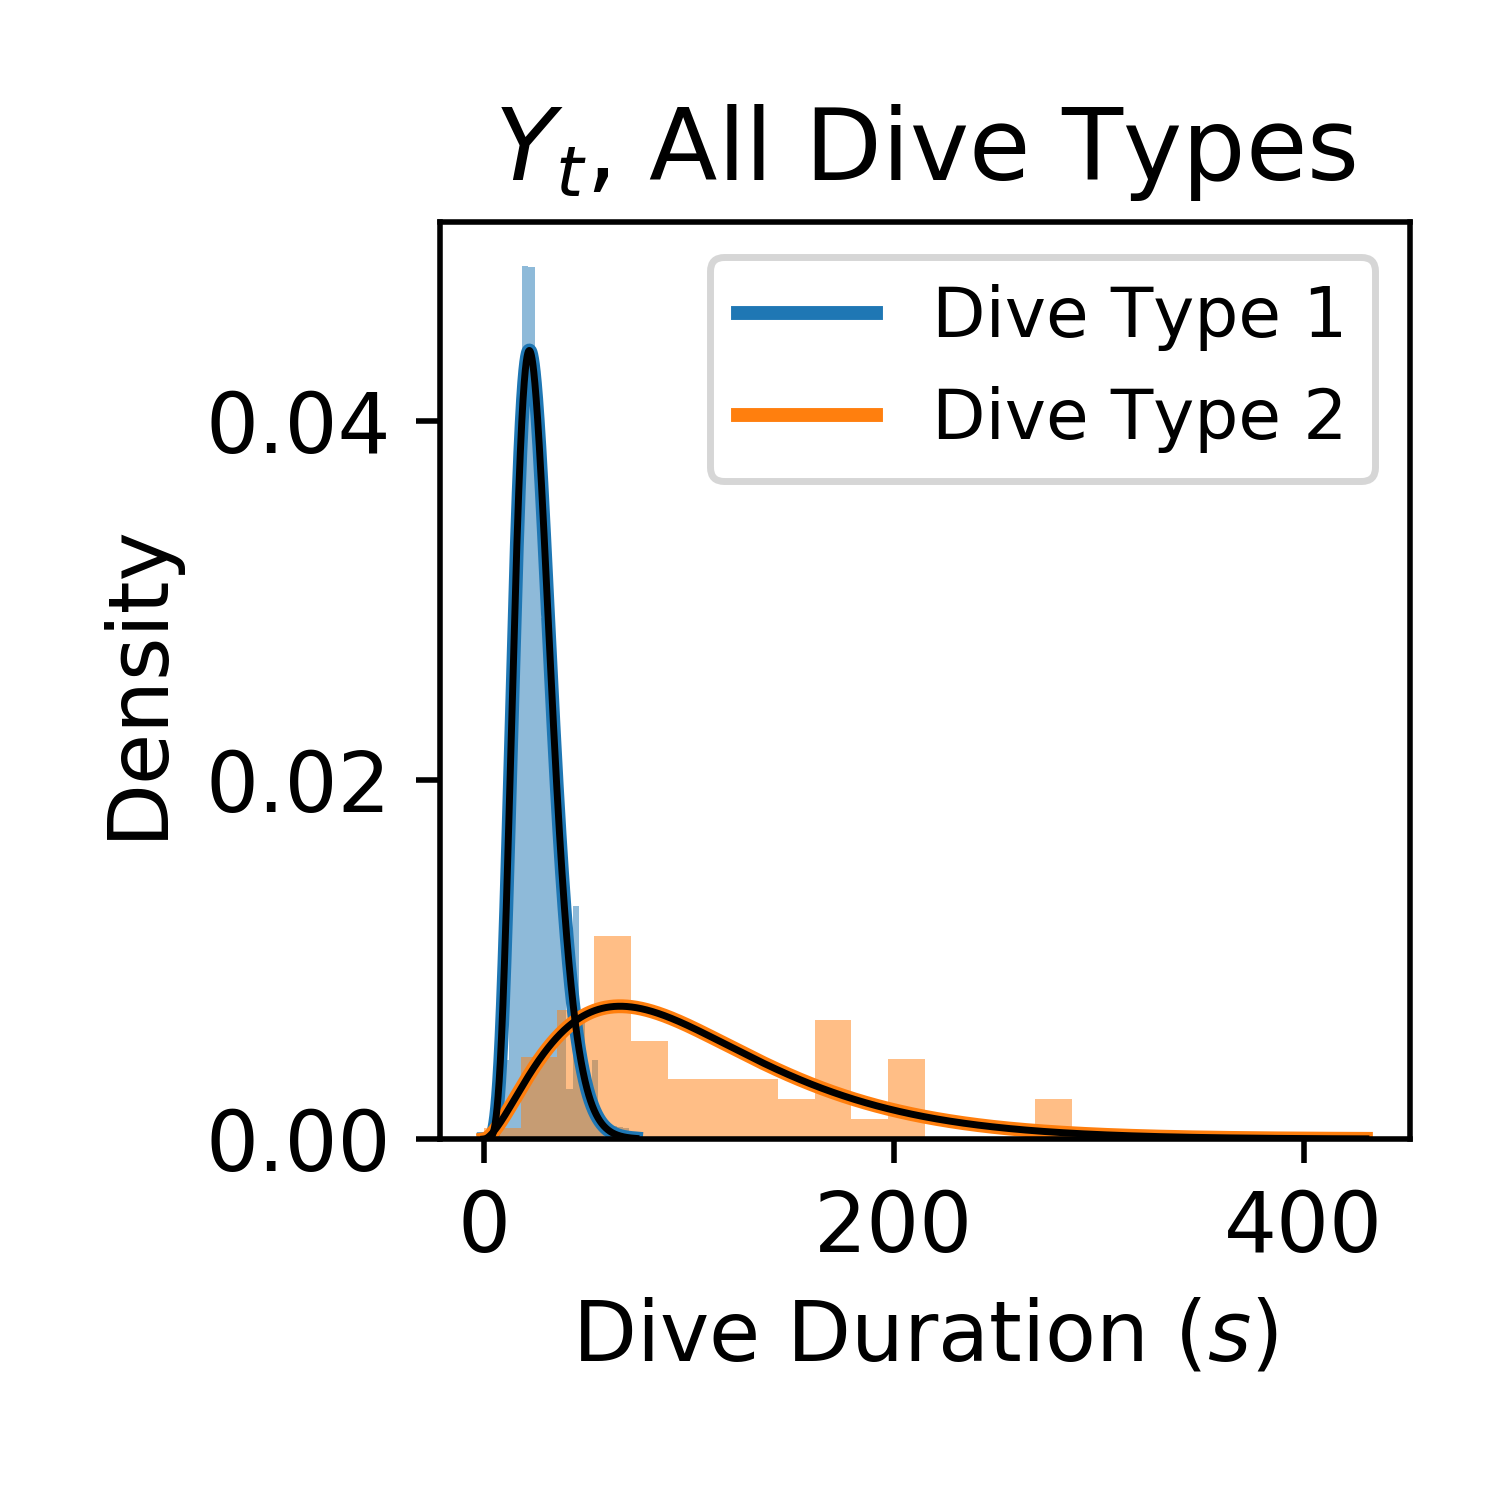
\includegraphics[width=2.25in]{../Plots/CarHHMM2_empirical_hist_dive_duration.png}
    	\caption{Empirical distribution of $Y$ (Dive Duration)}
    	\label{fig:empirical_dist}
    \end{subfigure}
    \caption{Examples of psuedoresiduals and a weighted empirical distribution as model checking tools}
    \label{fig:model_checking}
\end{figure}